\documentclass[11pt,a4paper]{article}
\usepackage[T1]{fontenc}
\usepackage{lmodern}
\usepackage[margin=30mm]{geometry}
\usepackage{graphicx}
\usepackage{amsmath,amssymb,amsthm}
\usepackage[hidelinks]{hyperref}
% Shared notation and theorem environments for this article.
\newtheorem{theorem}{Theorem}[section]
\newtheorem{proposition}[theorem]{Proposition}
\newtheorem{lemma}[theorem]{Lemma}
\newtheorem{corollary}[theorem]{Corollary}
\theoremstyle{definition}
\newtheorem{definition}[theorem]{Definition}
\newtheorem{example}[theorem]{Example}
\theoremstyle{remark}
\newtheorem{remark}[theorem]{Remark}
\newcommand{\R}{\mathbb R}
\newcommand{\Sph}{S^2}
\newcommand{\V}{\mathcal V_9}
\newcommand{\cH}{\mathcal H}
\newcommand{\normT}[1]{\left\lVert #1\right\rVert_{T_\eta}}
\newcommand{\dd}{\delta_\eta}
\newcommand{\aeta}{a_\eta}
\newcommand{\PP}{\mathsf P_\eta}
\DeclareMathOperator{\dist}{dist}

\hypersetup{
 pdftitle={Sup-norm stability radii for a nodal face of the B3 spherical discriminant},
 pdfauthor={Oleksiy Babanskyy},
 pdfsubject={Nodal graph stability in the full real spherical polynomial band}
}
\setlength{\emergencystretch}{1em}
\title{Sup-norm stability radii for a nodal face\\of the $B_3$ spherical discriminant}
\author{Oleksiy Babanskyy}
\date{}
\begin{document}
\maketitle

\begin{abstract}
How large can a real perturbation be before a nodal line ceases to be a
single graph in a fixed spherical sector? We study a truncated face of
the degree-nine $B_3$ discriminant, allowing all 100 real spherical
polynomial modes of degree at most nine and measuring the supremum norm
on the entire closed tube. The failure radius equals the minimum cost
of cancelling the field and its normal derivative. We bound it on the
full parameter domain and determine it exactly in two sufficient
regimes, using an explicit atomic mixed-jet certificate on the sphere.
In these exact regimes the unique critical field is a scaled Chebyshev
polynomial, and the whole closed radius ball still preserves the graph,
although the critical zero level is singular; every larger amplification
of that field fails. Two continuous examples separate the limits of a
support criterion from those of the radius formula. Below the radius
we obtain quantitative graph bounds. In the exact regimes a smooth
family approaching the critical field from inside the ball has uniformly convergent graphs and
terminal slopes diverging as $\varepsilon^{-1/3}$ at the minimizing
terminals. Persistence and $C^1$ conditioning therefore separate.
\end{abstract}

\section{Introduction}\label{sec:introduction}

The zero set of a signed field describes a geometric pattern. Its
stability depends on the permitted errors, the norm used to measure
them and the property one wants to preserve. Here the property is
particularly concrete: within a prescribed spherical tube, the entire
zero set must remain one interior $C^1$ graph over the angular interval.
The perturbation is measured only by its values, but belongs to a fixed
finite-dimensional band. This restriction allows a positive stability
radius; arbitrary smooth errors with small values need not preserve
the graph.

Our target is the product of the nine unit-normal mirror forms of
$B_3$, restricted to the unit sphere. We truncate one of its nodal faces
before its mirror intersections and work in a closed tube with two
normal sides and two angular terminal fibres. Perturbations use all
real spherical modes of degree at most nine, without symmetry
constraints. A smooth graph is permitted even when the field defining
its zero level has a vanishing gradient. This distinction is decisive
at the critical radius.

The analysis has three parts. First, the graph-failure radius reduces
to a variational cost for a value and an oriented normal derivative.
For this target the normal-side escape cost is strictly larger, and
the same minimum is obtained by setting both jet components to zero.
Second, a moving atomic formula on the sphere gives a sharp lower
bound in two geometric regimes, identifies every minimizing point
and the unique minimizing field, and proves safety of the entire
closed ball. Third, the margin below this radius controls graph
position and slope, but an explicit interior approach to the critical
field yields unbounded terminal slope despite uniform convergence
of the graphs. These are geometric assertions about signed fields;
no plate response, particle transport or material deposition is
assumed or certified.

\subsection{Relation to approximation and discriminant distances}

Atomic representations of functionals on finite-dimensional subspaces
of $C(K)$ and complementary sign saturation are classical; a useful
account is \cite[Section 4.2]{Dressler}. That work fixes the sum of the
highest-degree coefficients and constructs explicit alternating
Chebyshev atoms on diagonally determined sets
\cite[Theorem 4.8]{Dressler}. For prescribed nodes,
\cite[Theorem 9]{DavydovSchaback} relates exact formulas with
$\ell^1$ weights to dual $\ell^\infty$ bounds on sampled data.
These principles motivate the
certificate here. Its specific ingredients are a moving spherical
support for a mixed value--normal-derivative functional, a rational
interpolation cancellation on the complete band, and saturation in
the continuous tube norm. A single-functional formula does not imply
reconstruction of every field from its atoms, nor is a minimal number
of atoms asserted.

The complementary fibre bound uses the real trigonometric
value--derivative inequality of Erd\'elyi
\cite[Theorem 2.1]{Erdelyi}. We state the imported inequality and check
its interval and degree hypotheses in Section~\ref{sec:barrier}.
The remaining finite-dimensional separation, support and rigidity
arguments are proved in the article.

Distances to singularity discriminants provide a related viewpoint
with different norms and events. Raffalli computes the Bombieri
distance for homogeneous forms on the whole sphere and gives a
closest contact perturbation at a minimizing point
\cite[Theorems 5.1 and 5.4]{Raffalli}.
Kozhasov, Mourrain and Parusi\'nski express higher discriminant
distances through Taylor jets in the Bombieri--Weyl geometry
\cite[Proposition 3.2, equations (3.8)--(3.9)]{KozhasovMourrainParusinski}; their
Theorem 5.3 identifies a Chebyshev extremizer among real-rooted binary
forms with fixed norm. Our space contains every degree from zero
through nine and uses a supremum on a truncated tube. The global
$B_3$ target already has singular mirror intersections. Consequently,
the whole-sphere discriminant distance does not supply the positive
local radius studied here. The ordinary singularity event uses the
value and full tangential gradient; our jet event uses the value and
one normal derivative, with escape through the normal sides checked
separately.

Lerario and Stecconi obtain isotopy under a strict distance from
nontransversality in a differentiable norm and describe the scalar
$C^1$ distance on a closed disk using the value together with the full gradient in the interior
and its projection tangent to the boundary on the boundary
\cite[Lemma 20 and Proposition 31]{LerarioStecconi}.
Their boundary transversality and isotopy of pairs differ from the
fixed-fibre graph property on our tube with angular terminals and
corners. In the two exact regimes, the graph at our sharp threshold remains
smooth even though the defining level is singular. The comparison
identifies the role of the band, norm, domain and preserved property;
it does not transfer a conclusion between these settings.

\subsection{Organization}

Section~\ref{sec:problem} fixes the problem and states the main results.
Sections~\ref{sec:variational} and \ref{sec:dualandbounds} reduce
graph failure to a jet cost and give general bounds.
Section~\ref{sec:atomic} constructs the certificate; Section~\ref{sec:exact}
proves rigidity and the exact regimes. Section~\ref{sec:examples}
gives the two delimiting examples. Sections~\ref{sec:quantitative}
and \ref{sec:limits} treat conditioning and the scope boundaries.
Section~\ref{sec:discussion} summarizes the conclusions and the
autonomous computational companion. Appendix~\ref{app:harmonics}
justifies the full spherical-band description.

\section{Setting and main results}\label{sec:problem}

\subsection{Target, coordinates, and the closed tube}
Let $\Sph=\{(x,y,z)\in\R^3:x^2+y^2+z^2=1\}$. On this unit sphere,
the target is the product of nine unit-normal linear forms,
with multiplicative factor one:
\begin{equation}\label{eq:target}
 f(x,y,z)=\frac{xyz(x^2-y^2)(x^2-z^2)(y^2-z^2)}{8}.
\end{equation}
This convention does not set the supremum of $f$ to one.
The factor $1/8$ is part of the normalization: this is the product
of the nine unit-normal linear forms
\[
 x,\ y,\ z,\quad
 \frac{x-y}{\sqrt2},\ \frac{x+y}{\sqrt2},\quad
 \frac{x-z}{\sqrt2},\ \frac{x+z}{\sqrt2},\quad
 \frac{y-z}{\sqrt2},\ \frac{y+z}{\sqrt2}.
\]
We consider the open nodal face $z=0$, $x>y>0$ and then truncate it.
Fix
\begin{equation}\label{eq:domain}
 0<\eta<\omega<\frac{\pi}{4},\qquad
 I=[\eta,\omega],\qquad
 \dd=\arctan\frac{\sin\eta\cos\eta}{4},\qquad
 \aeta=\sin\dd.
\end{equation}
Dependence on the fixed upper endpoint $\omega$ is suppressed in the
notation. Define
\begin{equation}\label{eq:chart}
 X(\theta,r)=(\cos r\cos\theta,\cos r\sin\theta,\sin r),\qquad
 D_\eta=I\times[-\dd,\dd],\qquad T_\eta=X(D_\eta).
\end{equation}
Here $r$ is signed geodesic distance from the equator and increases toward
positive $z$. Since $\dd<\pi/2$ and $0<\theta<\pi/4$, the chart is
injective: its inverse on the tube is
$r=\arcsin z$, $\theta=\arctan(y/x)$. Its metric is
$dr^2+\cos^2r\,d\theta^2$. We distinguish the \emph{normal sides}
$r=\pm\dd$ from the two \emph{angular terminal fibres}
$\theta=\eta,\omega$. All four are included in the tube.

\subsection{Perturbation class and graph property}
We use the full real space
\begin{equation}\label{eq:space}
 \V=\{p|_{\Sph}:p\in\R[x,y,z],\ \deg p\le9\}
     =\bigoplus_{\ell=0}^{9}\cH_\ell(\Sph;\R),
 \qquad \dim\V=100.
\end{equation}
Here $\cH_\ell$ consists of restrictions of homogeneous harmonic
polynomials of degree $\ell$. The equality and dimension in
\eqref{eq:space} are justified in Section~\ref{sec:finite} and
Appendix~\ref{app:harmonics}. There is no symmetry constraint on the
perturbation, and it need not lie in the degree-nine eigenspace alone.
For $e\in\V$, write
\[
 F=f\circ X,\qquad E=e\circ X,\qquad G_e=F+E,\qquad
 \normT e=\max_{p\in T_\eta}|e(p)|.
\]
The maximum is over the \emph{entire closed tube}; it is not a maximum
over sampled points or over a single fibre. This quantity is a norm on
$\V$ by Lemma~\ref{lem:norm}.

\begin{definition}[The property to be preserved]\label{def:graph}
The property $\PP(e)$ holds if there is a function
$h\in C^1(I)$, with $-\dd<h(\theta)<\dd$ for every $\theta\in I$,
such that
\begin{equation}\label{eq:graph}
 \{p\in T_\eta:(f+e)(p)=0\}
 =\{X(\theta,h(\theta)):\theta\in I\}.
\end{equation}
At the two angular endpoints, $C^1$ means a continuous one-sided
derivative. The definition concerns \emph{all} zeros in $T_\eta$ and
requires strict interiority at the normal sides. It does not require the
level set of $f+e$ to be regular.
\end{definition}

The failure radius is the infimum
\begin{equation}\label{eq:rho}
 \rho_\eta=\inf\{\normT e:e\in\V,\ \PP(e)\text{ fails}\}.
\end{equation}
We introduce the lateral cost and the oriented-jet cost,
\begin{align}
 j_\eta&=\min_{\theta\in I}F(\theta,\dd),\label{eq:j}\\
 d_\eta&=\inf\left\{\normT e:
   \begin{array}{l}
    e\in\V,\ (\theta,r)\in D_\eta,\\[-2pt]
    G_e(\theta,r)=0,\quad \partial_rG_e(\theta,r)\le0
   \end{array}\right\}.\label{eq:d}
\end{align}
Both the field and the point are variables in \eqref{eq:d}. In
particular, the point is not fixed at the centre of a fibre or at an
angular endpoint. We initially write an infimum; its attainment is part
of the result.

\begin{theorem}[Finite variational reduction]\label{thm:main}
For every pair of parameters in \eqref{eq:domain}, $j_\eta$ and $d_\eta$
are finite and strictly positive. The infimum defining $d_\eta$ is a
minimum. Moreover,
\begin{equation}\label{eq:main}
 \boxed{\rho_\eta=\min\{j_\eta,d_\eta\}.}
\end{equation}
This is an equality of costs. A zero with nonpositive normal derivative
is not, by itself, equivalent to failure of Definition~\ref{def:graph}.
\end{theorem}

Thus the geometric question can be reduced to finitely many field
coefficients and a point in a compact two-dimensional domain. The norm
constraint remains a condition on a continuum. The theorem neither
evaluates $d_\eta$ in closed form nor substitutes a finite grid for that
constraint. Section~\ref{sec:threshold} specifies exactly what the
reduction does and does not imply at equality.


\subsection{General bounds and the exact-radius regimes}
Set $a=\aeta$, $\delta=\dd$, $L=\omega-\eta$, and define
\begin{equation}\label{eq:radiusdata}
 B(\theta)=\frac{\sin^3(2\theta)\cos(2\theta)}{64},\quad
 \beta=\min\{B(\eta),B(\omega)\},\quad
 A_*=\frac{a\beta}{9},\quad W(a)=\frac{11a}{10+a^2}.
\end{equation}
This $B$ is the normal derivative of the target on the central face,
as verified in \eqref{eq:B}. The Chebyshev polynomial used below is
$T_9(t)=\cos(9\arccos t)$ for $|t|\le1$, extended polynomially.

\begin{theorem}[Radius, minimizing fields and the safe threshold]\label{thm:radius}
For every geometry in \eqref{eq:domain},
\begin{equation}\label{eq:universalradius}
 \frac{A_*}{2\cos(\delta/2)}\le
 \rho_\eta=d_\eta\le A_*<j_\eta,\qquad j_\eta\ge\frac{63}{8}A_*.
\end{equation}
Moreover $d_\eta$ is also the least norm for the exact jet
$G_e=\partial_rG_e=0$ at a point of the closed tube.
Consider either of the following sufficient hypotheses:
\begin{description}
\item[Uniform regime L:] $\sin(L/4)\ge W(a)$.
\item[Adapted regime M:] there is $\eta<\theta_c<\omega$ such that
\begin{equation}\label{eq:Msummary}
 \sin((\omega-\theta_c)/2)\ge W(a),\qquad
 \min\{B(\theta_c),B(\omega)\}\ge2\cos(\delta/2)B(\eta).
\end{equation}
\end{description}
Under either hypothesis, $\rho_\eta=d_\eta=A_*$ and the unique
field occurring in a minimizing jet pair is
\begin{equation}\label{eq:critical}
 e_C(x,y,z)=-A_*T_9(z/a).
\end{equation}
In L the minimizing points are precisely $(\theta,0)$ at the angular
terminals where $B(\theta)=\beta$, including both terminals in a tie.
In M only $(\eta,0)$ minimizes and $A_*=aB(\eta)/9$.
Every field in the closed ball $\normT e\le A_*$ satisfies $\PP$.
The infimum of genuine failures is not attained, whereas
$\gamma e_C$ is a genuine failure for every $\gamma>1$.
\end{theorem}

The general conclusions follow from Propositions~\ref{prop:exactjet},
\ref{prop:jetonly} and \ref{prop:strongfloor}. The exact regimes and
threshold assertions are proved in Section~\ref{sec:sharp}.
The two hypotheses are sufficient criteria for the radius formula;
neither is asserted to describe the maximal possible geometry.
Example~\ref{ex:M} satisfies M while violating the uniform support
condition L. Example~\ref{ex:F} has $\rho_\eta<A_*$, so a formula
valid for every geometry cannot be inferred from these regimes.


\subsection{Conditioning before the threshold}
The gap to the radius gives quantitative control strictly below
the threshold. For a fixed geometry and
$\normT e\le m<d_\eta$, Proposition~\ref{prop:margin} gives
\[
 \partial_rG_e(\theta,h(\theta))\ge
 \kappa:=\frac{\cos\delta}{2a}(d_\eta-m)>0,
 \qquad \|h\|_\infty\le\frac{2m}{\beta}.
\]
It also bounds the slope using a finite derivative operator norm on
the fixed band and tube. In L or M, $d_\eta=A_*$ is explicit.
Theorem~\ref{thm:degeneration} shows a different phenomenon at equality:
fields $e_\varepsilon$ strictly inside the ball converge smoothly to
$e_C$, their graphs converge uniformly to zero, yet
$|h_\varepsilon'(\theta_*)|$ diverges like $\varepsilon^{-1/3}$
at each minimizing terminal. The critical graph itself is smooth.

\section{Variational characterization of graph failure}\label{sec:variational}

\subsection{Geometry and signs on the whole tube}\label{sec:signs}

We first establish the target estimates, including the entire boundary
of the tube.
Set
\[
 c=\cos\theta,\quad s=\sin\theta,\quad
 v=c^2s^2,\quad C(\theta)=\frac{cs(c^2-s^2)}8>0,\quad
 t=\tan r,\quad q=t^2.
\]
Substitution into \eqref{eq:target}, using $c^2+s^2=1$, gives
\begin{equation}\label{eq:F}
 F(\theta,r)=C(\theta)\frac{t(v-q+q^2)}{(1+q)^{9/2}}.
\end{equation}
In particular, $F$ is odd in $r$ and $F(\theta,0)=0$. Define
\begin{equation}\label{eq:B}
 B(\theta)=\partial_rF(\theta,0)
          =C(\theta)v
          =\frac{\cos^3\theta\sin^3\theta\cos2\theta}{8}>0.
\end{equation}

\begin{lemma}[Positive normal derivative]\label{lem:monotone}
On the entire closed rectangle $D_\eta$,
\begin{equation}\label{eq:monotone}
 \partial_rF(\theta,r)>\frac{B(\theta)}2>0.
\end{equation}
Consequently $j_\eta>0$, the unperturbed zero set in the tube is exactly
$r=0$, and $F(\theta,-\dd)=-F(\theta,\dd)$.
\end{lemma}
\begin{proof}
Differentiating \eqref{eq:F} with $dt/dr=1+t^2$, without division by
$t$, yields
\begin{equation}\label{eq:Q}
 \partial_rF=C(\theta)\frac{Q(v,q)}{(1+q)^{9/2}},\qquad
 Q(v,q)=v-(3+8v)q+11q^2-4q^3.
\end{equation}
Since $v=\tfrac14\sin^2(2\theta)$ increases on $(0,\pi/4)$,
\[
 0\le q\le\tan^2\dd=\frac{\sin^2\eta\cos^2\eta}{16}
       \le\frac v{16}\le\frac1{64}.
\]
The inequalities $3+8v\le5$ and $q^2(11-4q)\ge0$ imply
$Q(v,q)\ge v-5q\ge11v/16$. Also
\[
 (1+q)^{9/2}\le(65/64)^{9/2}<(65/64)^5<11/8,
\]
where the last inequality follows from
$8\cdot65^5=9282325000<11811160064=11\cdot64^5$.
Combining these bounds proves \eqref{eq:monotone}.
Oddness was already obtained from \eqref{eq:F}. Integrating the positive
derivative from zero to $\dd$ gives
\[
 F(\theta,\dd)>\tfrac12\dd B(\theta)>0.
\]
Continuity on the compact interval $I$ gives a positive minimum in
\eqref{eq:j}. Strict increase and the zero at $r=0$ give the remaining
claims.
\end{proof}

\begin{corollary}[Signs below the lateral cost]\label{cor:signs}
If $\normT e<j_\eta$, then, uniformly for $\theta\in I$,
\begin{equation}\label{eq:signs}
 G_e(\theta,-\dd)<0<G_e(\theta,\dd).
\end{equation}
\end{corollary}
\begin{proof}
The right-hand value is at least $j_\eta-\normT e>0$; by oddness of
$F$, the left-hand value is at most $-j_\eta+\normT e<0$.
No symmetry of $e$ is used.
\end{proof}

\subsection{The full finite-dimensional space and the minimum of the jet cost}
\label{sec:finite}

\begin{proposition}[A complete set of 100 coordinates]\label{prop:basis}
Each $e\in\V$ has a unique representation on the sphere of the form
\begin{equation}\label{eq:basis}
 e(x,y,z)=A(y,z)+xB(y,z),\qquad \deg A\le9,\quad\deg B\le8.
\end{equation}
The corresponding 55 monomials of $A$ and 45 monomials of $B$ form a
basis of $\V$.
\end{proposition}
\begin{proof}
In any ambient polynomial of degree at most nine, repeatedly replace
$x^2$ by $1-y^2-z^2$. This preserves its restriction to the sphere,
does not increase degree, and produces \eqref{eq:basis}.
For uniqueness, suppose the expression in \eqref{eq:basis} vanishes
on the sphere. At every point with $y^2+z^2<1$, evaluate it at the two
values $x=\pm\sqrt{1-y^2-z^2}$. Adding and subtracting gives
$A(y,z)=B(y,z)=0$ on the open disk. A polynomial vanishing on an open
set is identically zero: one may fix one coordinate on a small rectangle
and apply the one-variable zero theorem successively to its coefficients.
Thus all coefficients vanish. There are
$(9+1)(9+2)/2=55$ monomials of degree at most nine in two variables and
$(8+1)(8+2)/2=45$ of degree at most eight.
\end{proof}

\begin{lemma}[The tube norm and compact sublevels]\label{lem:norm}
For fixed parameters \eqref{eq:domain}, $\normT\cdot$ is a norm on
$\V$, and every set $\{e:\normT e\le M\}$ with $M<\infty$ is
compact in coefficient coordinates.
\end{lemma}
\begin{proof}
Only positive definiteness needs proof. The tube contains a nonempty
open subset $U$ of the sphere. If $e$ vanishes on $T_\eta$, it vanishes
on $U$. Its restriction to a great circle is a trigonometric polynomial
of degree at most nine: each ambient coordinate is linear in the sine
and cosine of the circle parameter. Such a polynomial that vanishes on
an open arc vanishes on the whole circle, since multiplication by
$\exp(9it)$ makes it an ordinary polynomial in $\exp(it)$ with infinitely
many roots. For any $q\in\Sph$, choose a point of $U$ not parallel to
$q$ and the great circle through them. That circle contains an open arc
in $U$, so $e(q)=0$. Hence $e$ is the zero function on the sphere.

For compactness, let $b_1,\ldots,b_{100}$ be the basis from
Proposition~\ref{prop:basis}. Evaluations at points of $T_\eta$ span
the dual of $\V$. Otherwise a nonzero field would be annihilated by
every such evaluation, contradicting positive definiteness. Select 100
linearly independent evaluations. The matrix
$M_{ij}=b_j(p_i)$ is invertible, and $\normT e\le M_0$ bounds every
coordinate of $(e(p_i))_{i=1}^{100}$ by $M_0$. It therefore bounds the
coefficient vector by application of $M^{-1}$. Finally,
\[
 \bigl|\normT{e_c}-\normT{e_{c'}}\bigr|
 \le\normT{e_c-e_{c'}}
 \le\sum_{j=1}^{100}|c_j-c'_j|\,\normT{b_j},
\]
so the sublevel set is closed. The result follows from compactness of
closed bounded sets in $\R^{100}$.
\end{proof}

The evaluation points above are a compactness argument, not a numerical
norming mesh or an algorithm for computing the sup. The bound on the
inverse matrix may depend on $\eta$ and $\omega$; no uniform bound as
the tube degenerates is asserted.

\begin{proposition}[Attainment of the oriented-jet cost]\label{prop:d}
The infimum in \eqref{eq:d} is attained by some pair
$(e_*,(\theta_*,r_*))$, and $d_\eta>0$.
\end{proposition}
\begin{proof}
The feasible set is nonempty: $e=-f\in\V$ makes $G_e$ and
$\partial_rG_e$ identically zero. Set $M_0=\normT f$. It suffices to
minimize over pairs in
\[
 \{e\in\V:\normT e\le M_0\}\times D_\eta
\]
satisfying the two jet conditions. This product is compact by
Lemma~\ref{lem:norm}. The conditions $G_e=0$ and
$\partial_rG_e\le0$ are closed, because value and derivative depend
continuously on coefficients and point. The norm is continuous, so it
attains a minimum on this nonempty closed subset. Candidates of norm
larger than $M_0$ cannot improve it, as the candidate $-f$ already has
norm $M_0$.
If the minimum were zero, positive definiteness would force $e_*=0$.
But $\partial_rF>0$ everywhere on $D_\eta$, which is incompatible
with the derivative constraint. Thus the minimum is strictly positive.
\end{proof}

\subsection{From oriented fibre zeros to a \texorpdfstring{$C^1$}{C1} graph}\label{sec:graph}

Injectivity of $X$ implies that one interior zero on each fibre gives a
set-theoretic graph. It also gives a continuous graph in this setting:
if $\theta_n\to\theta$, any subsequential limit of the roots lies in
$[-\dd,\dd]$, is a root at $\theta$ by continuity, and must equal
its unique root. This compactness argument does not supply a derivative.
The stronger hypothesis below supplies it, without assuming that $G_e$
is monotone away from its zeros.

\begin{lemma}[Fibre-to-graph lemma]\label{lem:graph}
Suppose \eqref{eq:signs} holds and
\begin{equation}\label{eq:positivezeros}
 G_e(\theta,r)=0\quad\Longrightarrow\quad
 \partial_rG_e(\theta,r)>0\qquad ((\theta,r)\in D_\eta).
\end{equation}
Then $\PP(e)$ holds, including both angular terminal fibres.
\end{lemma}
\begin{proof}
Fix $\theta$. The side signs give an interior zero by the intermediate
value theorem. Every zero is simple by \eqref{eq:positivezeros}, hence
isolated. The zero set of this fibre is compact and is disjoint from the
normal endpoints. It is finite: an infinite set would have an
accumulation point that is also a zero, contradicting simplicity there.
Every zero crosses from negative to positive as $r$ increases. If two
consecutive zeros existed, the function would be positive just after the
first and negative just before the second; continuity would give another
zero between them. This contradicts consecutiveness. Thus there is exactly
one zero, denoted $h(\theta)$.

For completeness, the local scalar implicit-function argument can be
made directly. At a zero $(\theta_0,r_0)$, continuity of the derivative
gives a small open rectangle on which $\partial_rG_e$ is bounded below
by a positive number. At $\theta_0$ choose two nearby normal values
around $r_0$ with opposite signs. Those signs persist on a smaller open
interval of $\theta$ values. The intermediate value theorem and strict
monotonicity on that rectangle give a unique local root. The preceding
compactness argument gives its continuity. Applying the mean value theorem
separately in the two variables to
\[
 G_e(\theta+t,h(\theta+t))-G_e(\theta,h(\theta))=0
\]
and letting $t\to0$ then gives
\begin{equation}\label{eq:hprime}
 h'(\theta)=-\frac{\partial_\theta G_e(\theta,h(\theta))}
                    {\partial_rG_e(\theta,h(\theta))}.
\end{equation}
The denominator stays positive locally, so this derivative is continuous.
Their restrictions to $I$ agree wherever they overlap, by fibrewise uniqueness.

The same argument applies at $\theta=\eta$ and $\theta=\omega$:
the field is a global polynomial restriction and the chart is defined on
an open neighbourhood of the closed rectangle. Apply the local argument
there and then restrict to $I$. This supplies the required one-sided
endpoint derivatives. The side signs exclude zeros on $r=\pm\dd$,
and fibrewise uniqueness accounts for all zeros in the tube.
\end{proof}

\begin{corollary}[A necessary event below $j_\eta$]\label{cor:event}
If $\normT e<j_\eta$ and $\PP(e)$ fails, there is a point of
$D_\eta$ at which $G_e=0$ and $\partial_rG_e\le0$.
\end{corollary}
\begin{proof}
Corollary~\ref{cor:signs} gives the side signs. The conclusion is the
contrapositive of Lemma~\ref{lem:graph}.
\end{proof}

\begin{example}[A singular level with a smooth graph]\label{ex:singular}
The field $e=-f+z^3$ belongs to $\V$ and gives
$G_e(\theta,r)=\sin^3r$. Its entire zero set in $T_\eta$ is the
smooth graph $r=0$, while $\partial_rG_e=0$ at every zero; indeed the
spherical gradient of $f+e=z^3$ vanishes there. This example shows why the jet condition is not a
pointwise characterization of failure. It is not being asserted to have
norm below $j_\eta$, to minimize $d_\eta$, or to identify an equality
case of the sharp radius.
\end{example}

\subsection{Proof of the reduction}\label{sec:reduction}

The existence and positivity assertions of Theorem~\ref{thm:main}
follow from Lemma~\ref{lem:monotone} and Proposition~\ref{prop:d}.
We prove the two inequalities for \eqref{eq:main} separately.

\subsubsection{Every failure costs at least \texorpdfstring{$\min(j_\eta,d_\eta)$}{min(j,d)}}
Let $e$ violate $\PP$. If $\normT e\ge j_\eta$, the desired lower
bound is immediate. Otherwise Corollary~\ref{cor:event} provides a
point satisfying the two jet constraints, so $\normT e\ge d_\eta$
by definition. Taking the infimum over genuine failures gives
\begin{equation}\label{eq:lower}
 \rho_\eta\ge\min\{j_\eta,d_\eta\}.
\end{equation}

\subsubsection{A genuine failure at the lateral cost}
Let $\theta_j\in I$ minimize $F(\theta,\dd)$. The constant field
$e=-j_\eta$ belongs to $\mathcal V_0\subset\V$, has norm
$j_\eta$, and produces
\[
 G_e(\theta_j,\dd)=0.
\]
This zero on a normal side violates strict interiority in
Definition~\ref{def:graph}. Hence
\begin{equation}\label{eq:upperj}
 \rho_\eta\le j_\eta.
\end{equation}
We have not assumed that the minimum occurs at $\theta=\eta$.

\subsubsection{Approaching the jet cost by genuine failures}
It remains to consider $d_\eta<j_\eta$. Choose a minimizing pair
$(e_*,(\theta_*,r_*))$ from Proposition~\ref{prop:d}. It satisfies
$|r_*|<\dd$: a zero on either normal side would require
\[
 |e_*(X(\theta_*,r_*))|=|F(\theta_*,r_*)|\ge j_\eta>d_\eta,
\]
which is impossible. Put $z_* = \sin r_*$ and, for $\varepsilon>0$,
define the global field
\begin{equation}\label{eq:correction}
 e_\varepsilon(x,y,z)=e_*(x,y,z)-\varepsilon(z-z_*).
\end{equation}
The correction is in $\mathcal V_1=\mathcal H_0\oplus\mathcal H_1$
and so remains in the original admissible space. At the selected point,
\begin{equation}\label{eq:negative}
 G_{e_\varepsilon}(\theta_*,r_*)=0,\qquad
 \partial_rG_{e_\varepsilon}(\theta_*,r_*)
 =\partial_rG_{e_*}(\theta_*,r_*)-\varepsilon\cos r_*<0.
\end{equation}
The value is unchanged, and $\cos r_*>0$ on this tube. On the
\emph{whole tube}, $|z|\le\aeta$ and $|z_*|<\aeta$, so
\begin{equation}\label{eq:costcorrection}
 \normT{e_\varepsilon}
 \le d_\eta+\varepsilon(\aeta+|z_*|)
 \le d_\eta+2\aeta\varepsilon.
\end{equation}
Choose
\begin{equation}\label{eq:eps}
 0<\varepsilon<\frac{j_\eta-d_\eta}{2\aeta}.
\end{equation}
The field $e_\varepsilon$ still has the strict side signs
\eqref{eq:signs}. By the negative derivative in \eqref{eq:negative},
there is a small $s>0$ for which
\[
 -\dd<r_*-s<r_*<r_*+s<\dd,\qquad
 G_{e_\varepsilon}(\theta_*,r_*-s)>0,
 \quad G_{e_\varepsilon}(\theta_*,r_*+s)<0.
\]
Together with the negative sign at $-\dd$ and positive sign at
$\dd$, the intermediate value theorem gives one zero in
$(-\dd,r_*-s)$ and another in $(r_*+s,\dd)$. Along with $r_*$,
these are three distinct interior zeros on the same fibre. Thus
$\PP(e_\varepsilon)$ genuinely fails. The argument is unchanged
if $\theta_*$ is either angular endpoint, since that entire fibre is
included in $D_\eta$.

Letting $\varepsilon\downarrow0$ in \eqref{eq:costcorrection} yields
$\rho_\eta\le d_\eta$. If instead $d_\eta\ge j_\eta$, the
lateral witness already suffices. Combining these facts with
\eqref{eq:lower} proves Theorem~\ref{thm:main}. In particular, the
proof never replaces an admissible global field by a freely chosen
one-variable perturbation of a single fibre.

\subsection{Equality, attainment, and the limits of the conclusion}
\label{sec:threshold}

\begin{proposition}[What happens at the threshold]\label{prop:attainment}
The reduction has the following consequences.
\begin{enumerate}
\item Every field of norm strictly less than $\rho_\eta$ satisfies
      $\PP$.
\item If $j_\eta\le d_\eta$, the constant field $-j_\eta$ realizes
      a genuine failure of norm $\rho_\eta=j_\eta$.
\item If $d_\eta<j_\eta$, the closed ball
      $\{e:\normT e\le d_\eta\}$ is safe if and only if every
      field that occurs in a minimizing pair for the jet problem satisfies
      $\PP$. In the same case, the infimum of genuine failures is attained
      if and only if some jet-minimizing field violates $\PP$.
\end{enumerate}
\end{proposition}
\begin{proof}
The first assertion is the defining property of an infimum, and the
second follows from the lateral witness. For the third, any failure of
norm at most $d_\eta$ is below $j_\eta$ and therefore has a feasible
jet by Corollary~\ref{cor:event}. Its norm is at least $d_\eta$ by
definition, so it equals $d_\eta$ and occurs in a minimizing pair.
Conversely, a jet-minimizing field that violates $\PP$ is a failure
of precisely that norm. These two implications prove both equivalences.
\end{proof}

This case distinction records the logic of the reduction.
Proposition~\ref{prop:jetonly} proves that only $d_\eta<j_\eta$
occurs in the present family. The classification in
Section~\ref{sec:sharp} then identifies a safe jet minimizer in the exact
regimes. Correction~\eqref{eq:correction} gives unsafe fields converging
to it in the same tube norm.

The distinction is substantive. The jet feasible set is closed and has
a minimizing pair. Definition~\ref{def:graph} allows singular levels,
so those facts alone do not make the failure set closed, do not settle
the closed-ball threshold, and do not provide a uniform $C^1$ conditioning
bound for the graph. Example~\ref{ex:singular} separates geometric
regularity of the graph from regularity of the defining level.

\paragraph{Mathematical and physical boundaries.}
The result is for real fields, the complete degree-at-most-nine space,
the stated normalization, and one closed truncated tube. It makes no
claim about the global nodal topology, vertices outside the tube,
arbitrary out-of-band errors, complex phasor zeros, modulus or RMS zeros,
material deposition, or the realization of every admissible perturbation
by a particular apparatus. No numerical search or physical experiment is
used in this proof. Finite dimensionality supplies compactness but leaves
the continuous sup constraint intact.


\paragraph{Route to the sharp result.}
The next sections prove the dual description, the complementary lower
bounds and central rigidity. They then classify the minimizing pairs
and prove closed-ball safety in the two exact regimes, followed by
the two examples. The quantitative graph bounds and their critical
limit are treated in Section~\ref{sec:quantitative}.

\section{Dual jet costs and tube-wide bounds}\label{sec:dualandbounds}

\subsection{Pointwise jet costs and their dual description}\label{sec:dual}

For the rest of the text abbreviate $a=\aeta$, $\delta=\dd$ and
$L=\omega-\eta$. At $p=(\theta,r)\in D_\eta$, let
$v_p(e)=E(\theta,r)$ and $\ell_p(e)=E_r(\theta,r)$. The pointwise cost is
\begin{equation}\label{eq:pointcost}
 D(p)=\min\{\normT e:e\in\V,\ v_p(e)=-F(p),\
                         \ell_p(e)\le-F_r(p)\}.
\end{equation}
The field $-f$ is feasible. The compactness argument of
Proposition~\ref{prop:d} applies with $p$ fixed, so this minimum exists
and is positive. The joint minimizing pair in that proposition gives
$d_\eta=\min_{p\in D_\eta}D(p)$; no regularity assertion about the
function $D$ is needed for this equality. Neither constraint in
\eqref{eq:pointcost} is removed by any symmetry projection.

For a real linear functional $h$ on $\V$, put
$\|h\|_* =\max_{\normT e\le1}|h(e)|$. This dual norm uses the whole
tube. A pair $\lambda\in\R$, $\mu\ge0$ with
$\|\lambda v_p+\mu\ell_p\|_*\le1$ gives
\begin{equation}\label{eq:weakdual}
 \normT e\ge-(\lambda v_p+\mu\ell_p)(e)
              \ge\lambda F(p)+\mu F_r(p)
\end{equation}
for every feasible field. In particular a multiplier of value equal to
zero does not remove the value constraint from the primal problem.

\begin{proposition}[Exact pointwise duality]\label{prop:dual}
At every $p\in D_\eta$,
\begin{equation}\label{eq:dualmax}
 D(p)=\max_{\lambda\in\R,\ \mu\ge0}
 \{\lambda F(p)+\mu F_r(p):
                  \|\lambda v_p+\mu\ell_p\|_*\le1\}.
\end{equation}
Both extrema are attained. For any optimal primal field and dual pair,
\[
 \mu\bigl(\ell_p(e)+F_r(p)\bigr)=0,\qquad
 -(\lambda v_p+\mu\ell_p)(e)=\normT e=D(p).
\]
\end{proposition}
\begin{proof}
We give the finite-dimensional separation argument directly.
The image $C$ of the unit ball under
$e\mapsto(v_p(e),\ell_p(e))$ is compact, convex and symmetric. It
contains zero in its interior: the fields $1$ and $z-\sin r$ have
independent images $(1,0)$ and $(0,\cos r)$, with $\cos r>0$.
For $0<s<D(p)$, the compact set $sC$ and the closed half-line
$H=\{(-F(p),w):w\le-F_r(p)\}$ are disjoint. Their distance is
positive and attained. The line orthogonal to the difference of a
closest pair strictly separates them, by the usual first-variation
inequalities for distance on convex sets.

Write the separating functional, oriented with its larger values on
$H$, as $\varphi(v,w)=-\lambda v-\mu w$. Its infimum on $H$ is
finite only when $\mu\ge0$. Normalize by
$\max_C\varphi=\|\lambda v_p+\mu\ell_p\|_*=1$, which is
positive because $C$ contains zero in its interior. Strict separation
gives $\lambda F(p)+\mu F_r(p)>s$. The feasible multiplier set is
compact: the linear map $(\lambda,\mu)\mapsto\lambda v_p+\mu\ell_p$
is injective, so its dual norm bounds the two coefficients. Letting
$s\uparrow D(p)$ and taking a convergent subsequence proves the reverse
inequality to \eqref{eq:weakdual} and attainment of the maximum.
The two inequalities in \eqref{eq:weakdual} must then both be equalities,
giving the displayed conclusions.
\end{proof}

An exact norm for a constructed functional need not make its objective
the maximum in \eqref{eq:dualmax}. The certificates below therefore give
lower bounds, except at the central points where a feasible field also
attains the bound.


\subsubsection{Exact and oriented jets}
\begin{proposition}[Active derivatives and normal-side costs]\label{prop:exactjet}
If $|r|<\delta$, then $D(\theta,r)>|F(\theta,r)|$.
Every optimal dual pair in \eqref{eq:dualmax} has $\mu>0$,
and every optimal primal field has $E_r=-F_r$.
At either normal side, $D(\theta,\pm\delta)=|F(\theta,\pm\delta)|$.
There an optimal field with $E_r=-F_r$ exists, although other optimal
fields have $E_r<-F_r$ and every optimal oriented-dual pair has $\mu=0$.
Consequently, on the entire closed tube,
\begin{equation}\label{eq:exactjetcost}
 D(p)=\min\{\normT e:e\in\V,\ G_e(p)=0,\ \partial_rG_e(p)=0\}.
\end{equation}
\end{proposition}
\begin{proof}
At an interior normal point, a feasible field of norm $|F(p)|$ would
attain a maximum of its absolute value along the fibre there, so
$E_r(p)=0$, contradicting $E_r(p)\le-F_r(p)<0$. If $F(p)=0$,
norm zero would force $e=0$, with the same contradiction.
Since $\|v_p\|_*=1$ (constant fields attain this value), a dual
optimum with $\mu=0$ could achieve at most $|F(p)|$.
Thus $\mu>0$, and Proposition~\ref{prop:dual} gives the derivative
equality for every primal optimum. These arguments include angular
terminals: only interiority along the normal coordinate is used.

For the sides use the exact target factors derived in
Section~\ref{sec:barrier}, equation~\eqref{eq:RS}:
\[
 R_\theta(q)=(1-q)^4-\frac{q(1-q)^2(1-2q)}{v_\theta},
 \qquad S_\theta=R_\theta+2qR_\theta'.
\]
The derivative of $q(1-q)^2(1-2q)$ is
$(1-q)(1-7q+8q^2)>0$ for $0\le q\le a^2<1/65$.
Hence $R_\theta'<0$ and \eqref{eq:RSbounds} gives
$0<S_\theta(a^2)<R_\theta(a^2)$.
For either $p=(\theta,\pm\delta)$ the global linear field
\[
 e_{\rm lin}=-F(\theta,\delta)\frac za
\]
has value $-F(p)$, norm $|F(p)|$ and normal derivative
$-B(\theta)\cos\delta\,R_\theta(a^2)<-F_r(p)$.
The opposite bound follows from the value constraint. With
$\kappa=S_\theta(a^2)/R_\theta(a^2)\in(0,1)$, the field
\[
 e_{\rm eq}=\kappa e_{\rm lin}+(1-\kappa)(-F(p))
\]
mixes this linear field with a constant. It retains the prescribed value,
has the exact normal derivative, and has norm at most $|F(p)|$ by
convexity, hence exactly $|F(p)|$. Complementarity with the strict
linear optimum forces $\mu=0$ for every optimal oriented-dual pair.
This proves equality of the two minimum values, not equality of
their sets of minimizers at the normal sides.
\end{proof}

\subsection{Target estimates and a complementary fibre barrier}\label{sec:barrier}

\subsubsection{Uniform target bounds on the original domain}
Write $v_\theta=\sin^2\theta\cos^2\theta$, as in Section~\ref{sec:signs},
and introduce the normalized normal coordinate $t=\sin r/a$.
The identity
\[
 a^2=\frac{v_\eta}{16+v_\eta}<\frac1{65},\qquad
 \frac{a^2}{v_\theta}<\frac1{16}
\]
holds throughout the original angular interval. Direct substitution of
$z=\sin r$ into \eqref{eq:target} gives
\begin{equation}\label{eq:RS}
 \begin{split}
 F(\theta,\arcsin z)&=B(\theta)zR_\theta(z^2),\qquad
 F_r(\theta,\arcsin z)=B(\theta)\sqrt{1-z^2}\,S_\theta(z^2),\\
 R_\theta(q)&=1-c_1q+c_2q^2-c_3q^3+c_4q^4,\qquad
 S_\theta(q)=R_\theta(q)+2qR_\theta'(q),\\
 (c_1,c_2,c_3,c_4)&=(4+1/v_\theta,\ 6+4/v_\theta,\
                         4+5/v_\theta,\ 1+2/v_\theta).
 \end{split}
\end{equation}
For example the unsimplified factor is
$(1-q)^2[(1-q)^2-q(1-q)/v_\theta+q^2/v_\theta]$, which expands
to $R_\theta$. Here $B(\theta)$ is the positive quantity in
\eqref{eq:B}. These are exact identities, not a truncation of the target.

For $0\le q\le a^2$, both remainders after the linear terms are
nonnegative, since
\[
 c_2-c_3q+c_4q^2\ge6+4/v_\theta-(4+5/v_\theta)/65>0,
\]
\[
 5c_2-7c_3q+9c_4q^2\ge30+20/v_\theta-(28+35/v_\theta)/65>0.
\]
Moreover $c_1a^2<4/65+1/16=129/1040<1/8$. Consequently
\begin{equation}\label{eq:RSbounds}
 R_\theta(a^2t^2)\ge1-t^2/8,\qquad
 S_\theta(a^2t^2)\ge1-3t^2/8>0\quad(|t|\le1).
\end{equation}
These estimates require no extra small-angle assumption or restriction
on perturbation coefficients. Put
\begin{equation}\label{eq:Atheta}
 A_\theta=\frac{aB(\theta)}9.
\end{equation}

\subsubsection{A trigonometric inequality and its application}
For a real trigonometric polynomial $Q$ of degree at most a positive integer $n$,
and $0<d<\pi$, Erd\'elyi's Theorem 2.1 gives, for $|r|<d$,
\begin{equation}\label{eq:erdelyi}
 |Q'(r)|^2+\beta_{n,d}(r)^2|Q(r)|^2
 \le\beta_{n,d}(r)^2\max_{|s|\le d}|Q(s)|^2,\qquad
 \beta_{n,d}(r)=\frac{n\cos(r/2)}
 {\sqrt{\sin^2(d/2)-\sin^2(r/2)}}.
\end{equation}
We use the author's 18-page manuscript \cite[Theorem 2.1, pp.~4--5;
proof, pp.~9--11]{Erdelyi}. Its width parameter is $d$, distinct from
our oriented-jet cost $d_\eta$.

For fixed $\theta$, every ambient monomial of degree at most nine
restricts to a trigonometric polynomial in $r$ of degree at most nine.
Thus \eqref{eq:erdelyi} applies to $E(\theta,\cdot)$ with $n=9$ and
$d=\delta$. Its fibre supremum is at most $\normT e$. At a feasible
jet, $E=-F$ and $|E_r|\ge F_r>0$, giving
\begin{equation}\label{eq:barrierK}
 D(\theta,r)\ge
 K(\theta,r):=\sqrt{F(\theta,r)^2+
                F_r(\theta,r)^2/\beta_{9,\delta}(r)^2}
       \quad(|r|<\delta).
\end{equation}
At $r=\pm\delta$ use instead $D\ge|F|$, from the value constraint.
Defining $K=|F|$ there makes this bound continuous. In particular
$K(\theta,0)=A_\theta/[2\cos(\delta/2)]<A_\theta$: this fibre
bound alone does not give the central value of $D$.

\begin{proposition}[Uniform complementary barrier]\label{prop:barrier}
For every point of the closed tube, with $u=t^2$,
\begin{equation}\label{eq:Qbarrier}
 \frac{D(\theta,r)^2}{A_\theta^2}\ge
 \mathcal Q(u):=81u(1-u/8)^2+
                 \frac{16}{65}(1-u)(1-3u/8)^2.
\end{equation}
Consequently
\begin{equation}\label{eq:barrierconsequences}
 D(\theta,r)\ge\frac4{\sqrt{65}}A_\theta
 \quad\hbox{everywhere},\qquad
 D(\theta,r)>A_\theta\quad\hbox{if }|t|\ge1/10.
\end{equation}
\end{proposition}
\begin{proof}
Set
$c=\sqrt{1-a^2u}$ and $c_\delta=\cos\delta$. In the interior,
\[
 \frac{c^2}{a^2}
 \frac{\sin^2(\delta/2)-\sin^2(r/2)}{\cos^2(r/2)}
 =\frac{c^2(1-u)}{(1+c)(c+c_\delta)}
 \ge\frac{16}{65}(1-u),
\]
because $c^2\ge c_\delta^2>64/65$ and the denominator is at most
$4$. Equations~\eqref{eq:RS}--\eqref{eq:barrierK} give
\eqref{eq:Qbarrier}. At the normal sides $u=1$, its second term is
zero and the separate value bound gives the same conclusion.

On $[0,1]$ the first summand of $\mathcal Q$ has derivative
$81(1-u/8)(1-3u/8)\ge2835/64$. The derivative of the second is
bounded below by $-(16/65)(1+3/4)=-28/65$. Hence
$\mathcal Q'>0$, and $\mathcal Q(0)=16/65$. Also
\[
 \mathcal Q(1/100)>
 \frac{81}{100}\left(\frac{99}{100}\right)^2+
 \frac{16}{65}\left(\frac{99}{100}\right)^3
 =\frac{67127049}{65000000}>1.
\]
These facts prove both assertions, including the angular terminals and
the normal sides.
\end{proof}


\subsubsection{The universal radius and a sharper floor}
The function $B$ has derivative
\begin{equation}\label{eq:Bprime}
 B'(\theta)=\frac{\sin^2(2\theta)}{32}
                 \bigl(3-4\sin^2(2\theta)\bigr).
\end{equation}
It increases strictly up to $\pi/6$ and decreases strictly afterwards.
Thus $B\ge\beta$ on $I$, and its minimum is reached only at those
endpoints which realize $\beta$.

\begin{proposition}[The normal-side event is never first]\label{prop:jetonly}
On the whole original domain,
$\rho_\eta=d_\eta\le A_*<j_\eta$ and $j_\eta\ge63A_*/8$.
Every minimizing jet pair is interior in the normal coordinate.
\end{proposition}
\begin{proof}
The field $e_C$ in \eqref{eq:critical} has norm $A_*$ and
at each $(\theta_*,0)$ with $B(\theta_*)=\beta$ satisfies
$E_C=-F=0$ and $(E_C)_r=-9A_*/a=-F_r$.
Therefore $d_\eta\le A_*$. At $r=\delta$,
\eqref{eq:RSbounds} gives $F(\theta,\delta)\ge7aB(\theta)/8$.
Minimizing in $\theta$ gives $j_\eta\ge63A_*/8>A_*$.
Theorem~\ref{thm:main} proves the assertion about $\rho_\eta$.
A point on a normal side costs at least $j_\eta$ by its value
constraint, so cannot occur in a minimizing pair.
\end{proof}

\begin{proposition}[A stronger all-point floor]\label{prop:strongfloor}
Put $g=[2(1+\cos\delta)]^{-1}$. For every point of the closed tube,
\begin{equation}\label{eq:strongfloor}
 \frac{D(\theta,r)^2}{A_\theta^2}\ge g+61t^2,\qquad
 D(\theta,r)\ge\frac{A_\theta}{2\cos(\delta/2)}.
\end{equation}
The second inequality is strict when $r\ne0$. In particular
$A_*/[2\cos(\delta/2)]\le\rho_\eta\le A_*$.
\end{proposition}
\begin{proof}
For $u=t^2$ and $c=\sqrt{1-a^2u}$, keep the exact derivative
factor from the preceding proof instead of replacing it by a constant:
\[
 \frac{c^2(1-u)}{(1+c)(c+\cos\delta)}
 \ge g(1-a^2u)(1-u).
\]
The denominator is at most $2(1+\cos\delta)$. Applying the target
bounds gives
\[
 \frac{D^2}{A_\theta^2}\ge
 81u(1-u/8)^2+
       g(1-a^2u)(1-u)(1-3u/8)^2.
\]
At $u=1$ the derivative term is zero and the value constraint gives
the same inequality. Since $(1-u/8)^2\ge49/64$ and
$\prod_i(1-x_i)\ge1-\sum_i x_i$ for $x_i\in[0,1]$, the last
display is at least
\[
 g+\left(\frac{3969}{64}-g(a^2+7/4)\right)u\ge g+61u.
\]
Indeed $g<1/2$ and $a^2+7/4<2$ make the coefficient greater
than $61$. Finally $\sqrt g=1/[2\cos(\delta/2)]$ and
$A_\theta\ge A_*$, while Proposition~\ref{prop:jetonly} supplies
the upper bound and the identity of costs.
\end{proof}

\begin{corollary}[Localization and reflection of minimizing points]\label{cor:location}
Every minimizing pair has $|t|<1/10$ and
$B(\theta)\le2\cos(\delta/2)\beta$, with the latter inequality
strict if $t\ne0$. Moreover $D(\theta,-r)=D(\theta,r)$.
\end{corollary}
\begin{proof}
The outer bound \eqref{eq:barrierconsequences} and $d_\eta\le A_*$
exclude $|t|\ge1/10$. The sharper floor gives the angular restriction.
The transformation $e(x,y,z)\mapsto-e(x,y,-z)$ preserves the space
and tube norm. At the reflected point it reverses the value and preserves
the normal derivative, exactly as required by the oddness of $F$ and
evenness of $F_r$. Applying it twice proves the equality of costs.
\end{proof}
In particular the sharper all-point floor complements, rather than
replaces, the $\mathcal Q$ barrier needed at $|t|=1/10$.

\section{The spherical atomic certificate}\label{sec:atomic}

\subsection{An atomic certificate on all 100 modes}\label{sec:lift}


The existence of a norm-preserving atomic formula for a functional
on a finite-dimensional subspace of $C(K)$, and the extremal sign
conditions at its atoms, are classical
\cite[Theorem 4.4, Corollary 4.5 and Proposition 4.7]{Dressler}.
At prescribed nodes, the relation between exact formulas and
minimal weight norms is described by
\cite[Section 3, Theorem 9]{DavydovSchaback}.
Representing one functional does not reconstruct every field
from those evaluations. Here the work is to exhibit supported
points and weights, prove the identity on the complete spherical
space and attain the continuous tube norm explicitly.

\subsubsection{A common geometric condition}
Fix $\tau=1/10$ and $r_t=\arcsin(at)$, $c_t=\sqrt{1-a^2t^2}$.
At an angular position $\theta$, choose a nonzero signed angle $\alpha$
such that the closed segment between $\theta$ and $\theta+\alpha$
lies in $I$. Assume
\begin{equation}\label{eq:supportcondition}
 \sin(|\alpha|/2)\ge W(a),\qquad W(a)=\frac{11a}{10+a^2}.
\end{equation}
In particular $|\alpha|\le L<\pi/4$. For each fixed $\theta,t,\alpha$,
with $|t|\le\tau$, define
\begin{equation}\label{eq:bq}
 \begin{gathered}
 w=e^{i\alpha}-1,\quad h=|w|^2=4\sin^2(\alpha/2),\qquad
 \\
 b_t(s)=\frac{1-a^2ts}{c_t},\quad
 q_t(s)=\frac{a^2(s-t)^2}{c_t^2h}\quad(-1\le s\le1).
 \end{gathered}
\end{equation}
All derivatives in $s$ below hold $\theta,t,\alpha$ fixed. In particular
they do not differentiate a choice of angular side with respect to its
centre. The positive affine function $b_t$ is tangent to
$c(s)=\sqrt{1-a^2s^2}$ at $s=t$:
\begin{equation}\label{eq:tangent}
 b_t(t)=c_t,\quad b_t'(t)=c'(t)=-a^2t/c_t,\quad
 b_t(s)^2-c(s)^2=\frac{a^2(s-t)^2}{c_t^2}.
\end{equation}

The following exact maximum determines reality of the intersections:
\begin{equation}\label{eq:maxdefect}
 \max_{|s|\le1,\ |t|\le\tau}
 \frac{a|s-t|}{1-a^2ts}=W(a).
\end{equation}
Indeed, for fixed $t$, the quotient without absolute value has derivative
$(1-a^2t^2)/(1-a^2ts)^2>0$ with respect to $s$. The maximum of the
absolute value is at $s=\pm1$. For $t\ge0$, the difference between
the two endpoint ratios, after removing $a$, is
$2t(1-a^2)/(1-a^4t^2)\ge0$, selecting $s=-1$. By reflection, the
maximum at fixed $t$ is $a(1+|t|)/(1+a^2|t|)$, strictly increasing
in $|t|$. Equality in \eqref{eq:maxdefect} occurs only at
$(s,t)=(-1,\tau),(1,-\tau)$.

\subsubsection{Points in the tube and conditional weights}
Let
\begin{equation}\label{eq:roots}
 S_\pm(s)=\frac{b_t(s)\pm\sqrt{b_t(s)^2-4q_t(s)}}2.
\end{equation}
Equations~\eqref{eq:supportcondition} and \eqref{eq:maxdefect} imply
that these are real and belong to $[0,b_t(s)]$, since
\[
 \frac{4q_t(s)}{b_t(s)^2}
 =\frac{1}{\sin^2(\alpha/2)}
   \left(\frac{a|s-t|}{1-a^2ts}\right)^2\le1.
\]
Use rotated coordinates $u=x\cos\theta+y\sin\theta$,
$v=-x\sin\theta+y\cos\theta$ and define points $Q_{s,\pm}$ by
\begin{equation}\label{eq:atoms}
 u+iv=b_t(s)+S_\pm(s)w,\qquad z=as.
\end{equation}
The quadratic equation for $S$ and \eqref{eq:tangent} give
$|u+iv|^2=1-a^2s^2$. Thus these are points on the original sphere.
For $0\le\xi\le1$ the argument of $1+\xi(e^{i\alpha}-1)$ lies
between $0$ and $\alpha$: its real part is positive and
\[
 \frac{\operatorname{Im}}{\operatorname{Re}}
 =\frac{\xi\sin\alpha}{1-\xi+\xi\cos\alpha}
\]
is monotone with the sign of $\alpha$. Taking $\xi=S_\pm/b_t$
proves $Q_{s,\pm}\in T_\eta$, even when $\theta$ is a terminal.
The auxiliary endpoints $b_t$ and $b_te^{i\alpha}$ themselves need
not lie on the sphere.

Define the probability measure
\begin{equation}\label{eq:conditional}
 \pi_{t,s}=\frac{S_+(s)}{b_t(s)}\delta_{Q_{s,-}}
                +\frac{S_-(s)}{b_t(s)}\delta_{Q_{s,+}}.
\end{equation}
At $s=t$, the roots are $0$ and $b_t(t)$, so the weights are $1$ and $0$.
For $s\ne t$ both weights are positive. At a repeated root the two
half-weights are added at their common point.

\subsubsection{Moment recurrence and both data of the jet}
For the distribution on the coordinate $S$ underlying
\eqref{eq:conditional}, its moments satisfy
\begin{equation}\label{eq:moments}
 m_0=1,\quad m_1=2q_t/b_t,\qquad
 m_n=b_tm_{n-1}-q_tm_{n-2}\quad(n\ge2).
\end{equation}
This follows from $S^2-b_tS+q_t=0$ and remains true at repeated roots.
Set $k_n=b_tm_n$. Then
\[
 k_0=b_t,\quad k_1=2q_t,\quad
 k_n=b_tk_{n-1}-q_tk_{n-2},\qquad \deg_s k_n\le n+1.
\]
The degree bound follows by induction from $\deg b_t\le1$ and
$\deg q_t\le2$. Hence
\begin{equation}\label{eq:rationalmoment}
\begin{aligned}
 R_m(t,s):=\int(u+iv)^m\,d\pi_{t,s}
 &=\sum_{n=0}^{m}\binom mn b_t(s)^{m-n}w^n m_n(s)\\
 &=\frac{P_{m+1}(s)}{b_t(s)},\qquad \deg P_{m+1}\le m+1.
\end{aligned}
\end{equation}
Because $q_t(t)=q_t'(t)=0$, \eqref{eq:moments} also gives
$m_n(t)=m_n'(t)=0$ for $n\ge1$. Thus
\begin{equation}\label{eq:momentjet}
 R_m(t,t)=c_t^m,\qquad
 \partial_sR_m(t,t)=m c_t^{m-1}c'(t).
\end{equation}

For completeness, the real and imaginary parts of
\begin{equation}\label{eq:fourierbasis}
 z^k(u+iv)^m,\qquad k+m\le9,
\end{equation}
with only the real part when $m=0$, form a basis of $\V$.
There are $10+2(9+8+\cdots+1)=100$ such functions. They are
independent: at fixed $z\in(-1,1)$, put
$u+iv=\sqrt{1-z^2}e^{i\phi}$. Fourier uniqueness in $\phi$ forces
each polynomial coefficient in $z$ to vanish; its nonzero spherical
factor $(1-z^2)^{m/2}$ can be divided out. Varying $z$ shows that
all coefficients vanish. Proposition~\ref{prop:basis} supplies the
dimension, so independence proves completeness.

For every real field $e\in\V$, equations
\eqref{eq:rationalmoment}--\eqref{eq:momentjet} imply
\begin{equation}\label{eq:fulljet}
 g_e(s):=\int e\,d\pi_{t,s}=\frac{P_e(s)}{b_t(s)},\quad
 \deg P_e\le10,\qquad
 g_e(t)=E(\theta,r_t),\quad
 g_e'(t)=\frac{a}{c_t}E_r(\theta,r_t).
\end{equation}
The factor $z^k=a^ks^k$ contributes its ordinary product-rule
derivative, so the statement includes every $k,m$ in
\eqref{eq:fourierbasis}. This reproduces the two original jet data.
It does not assert that an arbitrary field or its average is a free
polynomial of degree nine. The degree-ten numerator is retained and
handled next.

\subsubsection{Rational interpolation and signs}
Let $P=T_9$ and $U=U_8$, with their explicit forms
\begin{equation}\label{eq:chebyshev}
 \begin{split}
 P(s)&=9s-120s^3+432s^5-576s^7+256s^9,\\
 U(s)&=1-40s^2+240s^4-448s^6+256s^8,\qquad P'=9U,\\
 N(s)&=(s^2-1)U(s),\qquad s_j=\cos(j\pi/9),\quad
                         \sigma_j=(-1)^j\quad(0\le j\le9).
 \end{split}
\end{equation}
The elementary identity $P(\cos\phi)=\cos(9\phi)$ follows by
expanding the cosine recurrence. It gives $P(s_j)=\sigma_j$ and
$\max_{[-1,1]}|P|=1$. The ten $s_j$ are the simple roots of $N$.
Since $N$ has leading coefficient $256$ and the roots are decreasing,
$\operatorname{sign}N'(s_j)=\sigma_j$.

For $|t|\le\tau$, $U(t)\ge3/5-7/15625>1/2$, by discarding
the positive terms in its polynomial. Thus $N(t)<0$. Also
$\min_j|s_j|=\sin(\pi/18)>1/9$ by strict concavity of sine,
so $|s_j-t|>1/90$. Define
\begin{equation}\label{eq:lambdamass}
 \lambda(t)=-\frac{N'(t)}{N(t)}-\frac{a^2t}{1-a^2t^2},
 \qquad M(t)=P'(t)+\lambda(t)P(t).
\end{equation}
Writing $\kappa=b_t'(t)/b_t(t)=-a^2t/(1-a^2t^2)$, the
functional $J_tQ=Q'(t)+\lambda(t)Q(t)$ satisfies
$J_t(N/b_t)=0$. For the cardinal polynomials
$L_j(s)=N(s)/[(s-s_j)N'(s_j)]$, every polynomial $V$ of degree
at most ten has $V-\sum_jV(s_j)L_j$ equal to a constant times
$N$. Divide this identity by $b_t$ and apply $J_t$ to obtain
\begin{equation}\label{eq:rationalinterp}
 J_t(V/b_t)=\sum_{j=0}^{9}d_j(t)(V/b_t)(s_j),\qquad
 d_j(t)=\frac{b_t(s_j)}{c_t}
     \frac{-N(t)}{(t-s_j)^2N'(s_j)}.
\end{equation}
The expression for $d_j$ follows by differentiating
$b_t(s_j)L_j(s)/b_t(s)$; the $N'$ and $b_t'$ terms cancel
using the specified sign of $\kappa$. All denominators are nonzero and
\begin{equation}\label{eq:signweights}
 \sigma_jd_j(t)>0.
\end{equation}

\begin{theorem}[Full-space atomic representation]\label{thm:certificate}
Under \eqref{eq:supportcondition}, for every $|t|\le1/10$ and
every $e\in\V$, the functional
\begin{equation}\label{eq:originalJ}
 J_{\theta,t}(e)=\frac{a}{c_t}E_r(\theta,r_t)+
                                  \lambda(t)E(\theta,r_t)
\end{equation}
has the representation
\begin{equation}\label{eq:atomicJ}
 J_{\theta,t}(e)=\sum_{j=0}^{9}d_j(t)
 \left[\frac{S_+(s_j)}{b_t(s_j)}e(Q_{s_j,-})+
       \frac{S_-(s_j)}{b_t(s_j)}e(Q_{s_j,+})\right].
\end{equation}
Its exact norm is
\begin{equation}\label{eq:exactnorm}
 \|J_{\theta,t}\|_*=M(t)=\sum_{j=0}^{9}|d_j(t)|>0.
\end{equation}
The normalized original multipliers are
$\lambda_r=\lambda(t)/M(t)$ and $\mu_r=a/(c_tM(t))>0$.
\end{theorem}
\begin{proof}
Apply \eqref{eq:rationalinterp} to the degree-ten numerator in
\eqref{eq:fulljet}. The two matching data there identify its left-hand
side with \eqref{eq:originalJ}. At the contact nodes $q_t(s_j)>0$,
so both conditional weights are positive. The signed measure in
\eqref{eq:atomicJ} has total variation at most $\sum_j|d_j|$.
All its points lie in $T_\eta$, so this bounds the dual norm.

The global polynomial $p_*(x,y,z)=P(z/a)$ belongs to $\V$ and
has $\normT{p_*}=1$. At both points of level $s_j$ it equals
$\sigma_j$. Therefore
\[
 J_{\theta,t}(p_*)=\sum_jd_j\sigma_j=
                   \sum_j|d_j|=P'(t)+\lambda(t)P(t)=M(t)>0.
\]
This proves saturation and hence \eqref{eq:exactnorm}. Points at
different levels cannot coincide. If two points at the same level
coincide, their weights have the same sign and add, preserving total
variation and saturation. The chain factor $a/c_t$ is positive,
giving the asserted sign of $\mu_r$ for both signs of $t$.
\end{proof}

The proof verifies the identity on a basis of the full
100-dimensional real space and
uses the original tube norm. A positive combination of
\emph{signed contact evaluations} is not a functional positive on
every nonnegative field.

\subsubsection{Tangency, aggregation, and terminal positions}
If \eqref{eq:supportcondition} is strict, all twenty contact points
are distinct. On its equality boundary, \eqref{eq:maxdefect} shows
that a discriminant vanishes only for $(s,t)=(-1,\tau)$ or
$(1,-\tau)$. At that level $S_+=S_-=b_t/2$, so the two
half-weights form one atom. There are exactly nineteen atoms when
$|t|=\tau$, and twenty when $|t|<\tau$. This statement applies at
each angular centre whose chosen side has equality, including a
terminal; it is not restricted to the angular midpoint.

Although the individual square roots may fail to be differentiable in
parameters at tangency, the moment recurrence and rational expressions
are regular because $b_t>0$. Jet matching differentiates those moments,
not the individual roots. At $t=0$, separately, $\lambda(0)=0$,
$M(0)=9$ and $\mu_r=a/9$; the value constraint remains present.

\subsection{The objective estimate on the original geometry}\label{sec:objective}

We now prove the scalar estimate on the full parameter domain.
Its geometric premise is precisely
the support condition needed for Theorem~\ref{thm:certificate}; the
scalar estimates themselves hold for every original geometry.

\begin{lemma}[Uniform objective margin]\label{lem:objective}
For $|t|\le1/10$, let $R=R_\theta(a^2t^2)$ and
$S=S_\theta(a^2t^2)$. With \eqref{eq:lambdamass}, $0<M(t)<24$,
and
\begin{equation}\label{eq:objective}
 \frac{9(S+\lambda(t)tR)}{M(t)}=
 \begin{cases}
  1,&t=0,\\
  \displaystyle 1+\frac{\Delta_\theta(t)}{M(t)}
        >1+\frac{111}{8}t^2,&0<|t|\le1/10.
 \end{cases}
\end{equation}
Here $\Delta_\theta(t)=9(S+\lambda(t)tR)-M(t)>333t^2$
off centre.
\end{lemma}
\begin{proof}
Put $x=t^2\le1/100$. The explicit polynomials give, for $t\ne0$,
\[
 \begin{gathered}
 \tfrac12<U\le1,\qquad
 U-1\le x(-40+12/5+4/15625)<0,\\
 U'/t\le-80+48/5+32/15625<0,\\
 0<39/5-9/15625\le P/t<9.
 \end{gathered}
\]
The lower bound on $U$ was proved above; the lower bound on $P/t$
discards its positive terms, while its upper bound uses
$-120+108/25+4/15625<0$. Consequently
\[
 \frac{\lambda(t)}t=
 \frac2{1-x}-\frac{U'(t)/t}{U(t)}-
                \frac{a^2}{1-a^2x}>2-\frac1{64}=\frac{127}{64}>0.
\]
Also
\[
 0<-tU'(t)=x(80-960x+2688x^2-2048x^3)<81x,
\]
since $80+2688/10000<81$. It follows that
$0<\lambda(t)t<3x+162x=165x$, and hence
\[
 0<M(t)=9U+(\lambda t)(P/t)<9+1485x\le477/20<24.
\]

Using \eqref{eq:RSbounds},
\[
 S-U\ge x(317/8-12/5-4/15625)>37x,
\]
\[
 9R-P/t\ge x(951/8-108/25-4/15625)>114x.
\]
The final strict inequalities follow respectively from
$9/40>4/15625$ and $111/200>4/15625$. Since $\lambda t>0$,
\[
 \Delta_\theta(t)=9(S-U)+(\lambda t)(9R-P/t)>333x.
\]
Dividing by $0<M<24$ gives \eqref{eq:objective}, because
$333/24=111/8$. At $t=0$, substitution gives $R=S=U=1$,
$P=\lambda=0$ and $M=9$, without division by $t$. This also
proves the mass bound at the centre. The estimates use
\eqref{eq:RSbounds}, which holds throughout the stated parameter domain.
\end{proof}

\begin{corollary}[Certified pointwise lower bounds]\label{cor:pointlower}
Where \eqref{eq:supportcondition} holds,
\begin{equation}\label{eq:pointlower}
 D(\theta,r_t)>A_\theta(1+111t^2/8)
                  \quad(0<|t|\le1/10),\qquad
 D(\theta,0)=A_\theta.
\end{equation}
\end{corollary}
\begin{proof}
For every feasible field, \eqref{eq:exactnorm} and the positivity of
$a/c_t$ imply
\[
 \normT e\ge-\frac{J_{\theta,t}(e)}{M(t)}
 \ge\frac{(a/c_t)F_r+\lambda(t)F}{M(t)}
 =\frac{aB(\theta)(S+\lambda(t)tR)}{M(t)}.
\]
Take the infimum and use Lemma~\ref{lem:objective}. The value
constraint is an equality, so its transfer permits either sign of
$\lambda$. The inequality uses the positive derivative multiplier;
$\lambda t>0$ was used in the scalar objective estimate. At
$t=0$ the lower bound is attained by the global field
$e=-A_\theta P(z/a)$: its value is zero, its normal derivative is
$-B(\theta)$, and its tube norm is $A_\theta$. This proves the
pointwise central equality, without classifying all its minimizers.
\end{proof}

\section{Rigidity and exact stability regimes}\label{sec:exact}

\subsection{Central rigidity and two support regimes}\label{sec:regimes}


\subsubsection{Central rigidity, including its angular boundary}\label{sec:centralrigidity}
The central rigidity argument includes an available side of length
exactly $2\delta$ by distinguishing
the auxiliary chord from the locations of its actual contact atoms.

\begin{lemma}[A closed angular-side condition gives central rigidity]\label{lem:rigidity}
Fix $\theta_0\in I$. If one of its available angular sides has
length $b_*\ge2\delta$, then
\[
 D(\theta_0,0)=A_{\theta_0},\qquad
 e=-A_{\theta_0}p_*\quad\text{is its unique minimizer in }\V.
\]
\end{lemma}
\begin{proof}
Write $\varepsilon\in\{-1,1\}$ for the direction of the available
side and $\ell=|\alpha|$ for an auxiliary chord angle. At $t=0$
the kernel has
\[
 b_0(s)=1,\qquad q_0(s)=\frac{a^2s^2}{4\sin^2(\ell/2)},\qquad
 S_\pm(s)=\frac{1\pm\sqrt{1-4q_0(s)}}2.
\]
Reality for every $|s|\le1$ needs only $\ell\ge2\delta$.
The coordinates $z=as$ and $1+S_\pm(e^{i\varepsilon\ell}-1)$
give points on the sphere, since their horizontal squared modulus
is $1-a^2s^2$. At $\ell=2\delta$ the ten contact levels
$s_j=\cos(j\pi/9)$ are all nonzero, hence
$0<S_-(s_j)\le S_+(s_j)<1$.
Every contact therefore has angle strictly between $\theta_0$
and $\theta_0+2\varepsilon\delta$, even if that is the entire
available side. At $s_j=\pm1$ the roots coincide at $1/2$,
with angular offset $\varepsilon\delta$; these normal-side
points are included in the tube. Aggregation gives eighteen atoms,
distinct from the nineteen-atom tangencies on the strip boundary.

There are finitely many contact levels. By continuity their angles
remain in the physical side for every
$2\delta<\ell<2\delta+\epsilon<\pi/4$, for some $\epsilon>0$,
even when the auxiliary chord endpoint lies beyond that side.
The roots remain real for all $|s|\le1$. The moment and
interpolation identities are identities for global polynomial
fields on the sphere; their algebra does not require the
intermediate, noncontact points to lie in the tube.
Only the atoms used to bound the functional by the tube norm
must lie there, as just proved.

For completeness, at $t=0$ the conditional moments obey
$m_0=1$, $m_1=2q_0$, and
$m_n=m_{n-1}-q_0m_{n-2}$. Thus $\deg m_n\le n+1$,
and $m_n(0)=m_n'(0)=0$ for $n\ge1$.
On every Fourier--$z$ basis element the averaged function has
degree at most ten and derivative $aE_r(\theta_0,0)$ at zero.
Its interpolation remainder at the ten levels is a multiple
of the even polynomial $N(s)=(s^2-1)U_8(s)$, whose derivative
at zero vanishes. The same coefficients
\[
 d_j=\frac{-N(0)}{s_j^2N'(s_j)},\qquad
 \operatorname{sgn}d_j=(-1)^j
\]
therefore represent $a\ell_{(\theta_0,0)}$ for all the chord
angles just described. The two conditional weights are positive,
and evaluation on $p_*=T_9(z/a)$ shows that the mass and norm
are exactly $\sum_j|d_j|=T_9'(0)=9$.
This proves the lower cost $A_{\theta_0}$; the field
$-A_{\theta_0}p_*$ attains it with value zero.

Normalize any minimizer by $h=-e/A_{\theta_0}$. Then
$\normT h=1$ and $a\,\partial_r(h\circ X)(\theta_0,0)\ge9$ by feasibility;
the norm of the functional forces equality.
In each representation every signed contact value equals one,
since their positive weighted sum equals its full mass.
Put $z_j=as_j$, $R_j=\sqrt{1-z_j^2}$. The farther contact
has angular offset $\varepsilon\Psi_j(\ell)$, where
\[
 \Psi_j(\ell)=\frac{\ell}{2}
     +\arccos\frac{\cos(\ell/2)}{R_j},\qquad
 \Psi_j'(\ell)=\frac12+
   \frac{\sin(\ell/2)}{2\sqrt{\sin^2(\ell/2)-z_j^2}}>0.
\]
This follows by rotating the chord by $-\varepsilon\ell/2$;
its real part becomes $\cos(\ell/2)$.
For $\ell>2\delta$ in the above interval every farther contact
traces an open angular arc within the tube. Thus $h-p_*$
vanishes on an arc at each of the ten heights $z_j$.
At fixed height it is a trigonometric polynomial of degree at
most nine, so it vanishes on the entire latitude.
In \eqref{eq:fourierbasis} the coefficient at frequency $m$
has a polynomial factor of degree at most $9-m$, times the
nonzero factor $(1-z^2)^{m/2}$. Ten distinct roots force every
coefficient to vanish. Hence $h=p_*$ on the sphere.
\end{proof}

\subsubsection{A uniform side throughout the sector}
If
\begin{equation}\label{eq:Lcondition}
 \sin(L/4)\ge W(a),
\end{equation}
choose $\alpha=L/2$ for $\theta\le(\eta+\omega)/2$ and
$\alpha=-L/2$ otherwise. Every chosen segment lies in $I$ and
\eqref{eq:supportcondition} holds. Thus the central bound
\eqref{eq:pointlower} applies at every angle, and the barrier
\eqref{eq:barrierconsequences} covers $|t|\ge1/10$. Both bounds
apply at $|t|=1/10$. The side selection may jump at the angular
midpoint, but both choices represent the same functional and exact norm;
no globally continuous selection of atoms is asserted.
Since $B$ has its minimum on $I$ at an endpoint, these two overlapping
bounds imply the global lower bound
\begin{equation}\label{eq:Llower}
 d_\eta\ge\frac a9\min\{B(\eta),B(\omega)\}.
\end{equation}
The single-maximum property of $B$ follows from the derivative
computed immediately before Proposition~\ref{prop:jetonly}.

Condition~\eqref{eq:Lcondition} is necessary and sufficient for reality
of all intersections of this particular uniform-side construction:
if it fails, $(s,t)=(-1,1/10)$ has negative discriminant for each
chosen side. This does not exclude other certificates or imply a
smaller nodal-stability radius. Moreover $W(a)>a=\sin\delta$, so
\eqref{eq:Lcondition} implies $L>4\delta$, even on its equality
boundary. In particular Lemma~\ref{lem:rigidity} applies at
every centre, using a side of length at least $L/2>2\delta$.


\subsubsection{A local side and a closed target margin}
Let $\eta<\theta_c<\omega$ and suppose
\begin{equation}\label{eq:Mcondition}
 \sin((\omega-\theta_c)/2)\ge W(a),\qquad
 \min\{B(\theta_c),B(\omega)\}\ge2\cos(\delta/2)B(\eta).
\end{equation}
For $\theta\in[\eta,\theta_c]$ choose $\alpha=\omega-\theta$.
The first condition qualifies the atomic construction on this
entire zone, including its cutoff, both strip edges and support
tangencies. The outer barrier covers $|t|\ge1/10$.
The second condition supplies the target margin on the complementary
angular zone, with its closed boundary treated separately below.

In the open second zone $(\theta_c,\omega)$ strict unimodality
gives $B(\theta)>\min\{B(\theta_c),B(\omega)\}$.
Proposition~\ref{prop:strongfloor} therefore gives $D>A_\eta$.
At either endpoint $\theta=\theta_c,\omega$ the strict
off-centre floor gives the same conclusion for $r\ne0$.
For the two remaining centres note that $W(a)>a=\sin\delta$,
so $\omega-\theta_c>2\delta$. From $\theta_c$ the side toward
$\omega$ is long enough for Lemma~\ref{lem:rigidity}; from
$\omega$ the side toward $\eta$ has length $L>2\delta$.
It follows that $D(\theta_c,0)=A_{\theta_c}>A_\eta$ and
$D(\omega,0)=A_\omega>A_\eta$, since $2\cos(\delta/2)>1$.
We have proved, including the equality in the target margin,
\begin{equation}\label{eq:Mright}
 D(\theta,r)>A_\eta
 \quad(\theta_c\le\theta\le\omega,\ |r|\le\delta).
\end{equation}
Thus no atom construction is needed to cover the open second zone;
the two endpoint centres use only the central cost lemma.
A strict lower bound of $\sqrt{65}B(\eta)/4$ or a lower bound
of $2B(\eta)$ for $\min\{B(\theta_c),B(\omega)\}$ each implies the
target-margin condition in \eqref{eq:Mcondition}.

On $[\eta,\theta_c]$ strict unimodality and $B(\theta_c)>B(\eta)$
give $B(\theta)>B(\eta)$ for $\eta<\theta\le\theta_c$.
The central-strip certificate and outer barrier then show
\begin{equation}\label{eq:Mlower}
 d_\eta\ge A_\eta.
\end{equation}
The closed regions overlap at $\theta_c$ and the normal
bounds overlap at $|t|=1/10$; no unexamined seam remains.
The support premise already implies $L>2\delta$ and does
not require $L>4\delta$.

\begin{figure}[tbp]
\centering
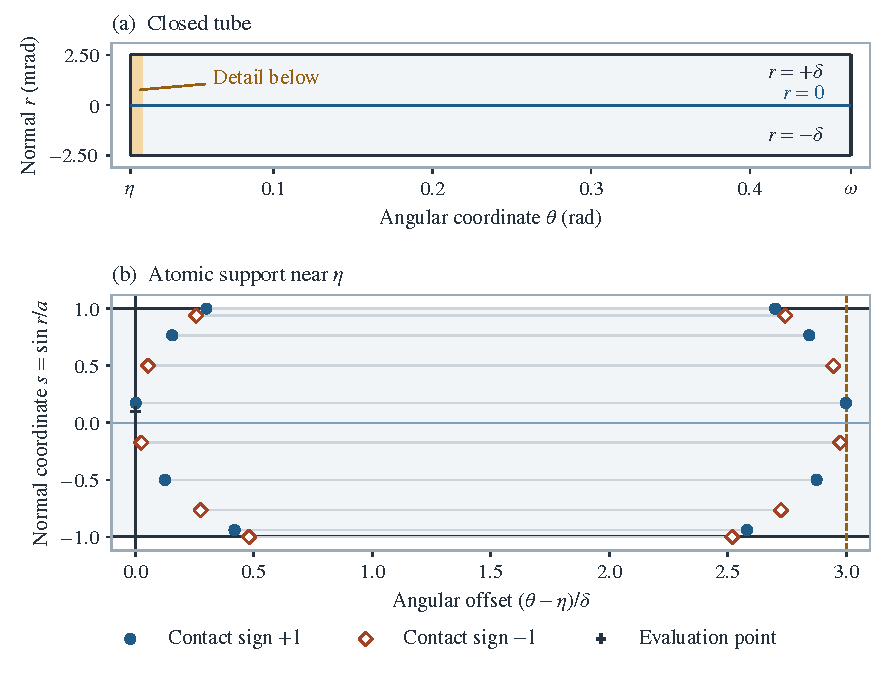
\includegraphics[width=\linewidth]{figures/tube_support.pdf}
\caption{The tube and an explicit supported jet, in coordinate charts.
Here $\eta=\arctan(1/100)$, $\omega=\arctan(1/2)$.
(a) The full angular interval and signed normal distance, with
independent axis scales; this is not an isometric development of
the sphere. (b) The twenty signed contacts of
Theorem~\ref{thm:certificate} at $\theta_0=\eta$, $t=1/10$,
using $\alpha=3\delta$, in coordinates
$((\theta-\eta)/\delta,\sin r/a)$.
The signs label the functional weights. The support count is
not asserted minimal, and the drawing is not a norm certificate.}
\label{fig:tube}
\end{figure}
The plotted case is qualified without numerical sampling:
$\eta<1/100$ and $\omega>2/5$ imply $L>39/100$, whence
$\sin(L/4)>9/100$, whereas $W(a)<11\eta/40<11/4000$.
Also $\delta<1/8$ gives
$\sin(3\delta/2)>(11/10)\delta>W(a)$ and $3\delta<L$.
Thus both the uniform regime and the inset side are admissible.
For these parameters $\sin(2\eta)<1/50$ and $B(\omega)=3/625$, so
$B(\eta)<(1/50)^3/64<3/625=B(\omega)$.
Thus $\eta$ is the minimizing terminal used in Figure~\ref{fig:fibre}.

\subsection{Exact radii and behaviour at equality}\label{sec:sharp}

\subsubsection{Classifying all minimizing pairs}
Under L, the strip certificate and the outer barrier give
$D(\theta,r)>A_\theta$ whenever $r\ne0$.
At $r=0$, every angle has an available side of length at least
$L/2>2\delta$, so Lemma~\ref{lem:rigidity} gives
$D(\theta,0)=A_\theta$ with the unique field
$-A_\theta T_9(z/a)$. Since $B$ has no interior minimum,
the minimizing points are exactly the terminal centres that
realize $\beta$. The minimum cost is $A_*$ and all those
points have the same unique minimizing field $e_C$.
This includes a tie between the two terminal fibres.

Under M, \eqref{eq:Mright} excludes the entire second zone.
In the first zone the same two bounds exclude $r\ne0$,
and $B(\theta)>B(\eta)$ for $\theta>\eta$ excludes the other
centres. Lemma~\ref{lem:rigidity} applies at $\eta$, giving
the only minimizing pair $((\eta,0),e_C)$ and cost
$A_\eta=A_*$. In both cases Proposition~\ref{prop:jetonly}
identifies this cost with $\rho_\eta$.

\subsubsection{The critical graph and the closed ball}
\begin{proposition}[The critical field and every amplification]\label{prop:criticalgraph}
For every original geometry the only zeros of $f+e_C$ in the
tube are $r=0$. At any terminal where $B=\beta$, the defining
level has zero spherical gradient there. For every $\gamma>1$,
$f+\gamma e_C$ has at least three distinct interior zeros on
each such terminal fibre.
\end{proposition}
\begin{proof}
The identity
\[
 1-\frac{T_9(t)}{9t}=t^2H(t^2),\qquad
 H(u)=\frac{40}{3}-48u+64u^2-\frac{256}{9}u^3
\]
extends continuously to $t=0$. Its derivative satisfies
$H'(u)=-(256/3)(u-3/4)^2\le0$, so
$H(u)\ge H(1)=8/9$ for $0\le u\le1$.
Using $B\ge\beta$ and the positive target bound yields, for
$r>0$ and $t=\sin r/a$,
\begin{equation}\label{eq:criticalsign}
 \frac{F+E_C}{\sin r}
 =B(\theta)R_\theta(a^2t^2)
       -\beta\frac{T_9(t)}{9t}
 \ge\frac{55}{72}\beta t^2>0.
\end{equation}
Oddness gives the opposite sign for $r<0$. Along the centre,
the angular derivative is zero and the normal derivative is
$B(\theta)-\beta$, proving the gradient assertion.

On a terminal with $B=\beta$, the field $F+\gamma E_C$
vanishes at the centre with derivative $(1-\gamma)\beta<0$.
It is negative just to its right. At
$t_0=\sin(\pi/9)\in(0,1)$, the first positive zero of $T_9$,
its value equals the strictly positive $F$.
The intermediate value theorem gives another positive zero
strictly between the centre and $t_0$. Oddness gives a
negative zero as well. This argument places no upper bound on
$\gamma$ and does not use normal-side signs.
\end{proof}

\begin{proof}[Completion of Theorem~\ref{thm:radius}]
The general bounds and the exact-jet identity were proved in
Propositions~\ref{prop:jetonly}, \ref{prop:strongfloor} and
\ref{prop:exactjet}. The preceding classification proves the
exact L/M radii and all their minimizing pairs.
If a field of norm at most $A_*<j_\eta$ failed $\PP$, then
Corollary~\ref{cor:event} would supply a feasible oriented jet.
Its norm would have to equal the minimum $A_*$, and the field
would have to be $e_C$. But Proposition~\ref{prop:criticalgraph}
shows that $e_C$ preserves the graph. The entire closed ball
is therefore safe. The fields $\gamma e_C$ have norms
$\gamma A_*$ and fail for every $\gamma>1$; as $\gamma$
decreases to one their costs approach $A_*$.
Thus the failure infimum is not attained in these regimes.
\end{proof}

\begin{figure}[tbp]
\centering
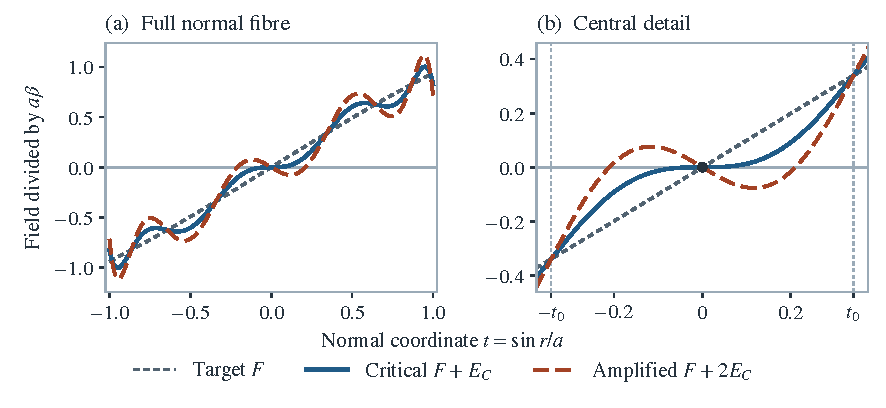
\includegraphics[width=\linewidth]{figures/fibre_threshold.pdf}
\caption{The terminal fibre $\theta=\eta$ for the same geometry
as Figure~\ref{fig:tube}. The horizontal coordinate is $t=\sin r/a$;
values are divided by $a\beta$. Curves show the target
$F$ and the perturbed fields $F+\gamma E_C$ with $\gamma=1,2$.
The second panel enlarges the central interval.
The guides $t=\pm\sin(\pi/9)$ are zeros of $T_9$, used as
sign witnesses in Proposition~\ref{prop:criticalgraph};
they are not the outer roots of the amplified field.
The curves illustrate the continuous proof; the conclusion
of at least three zeros follows from the proposition.}
\label{fig:fibre}
\end{figure}

The critical graph is smooth although its defining level is
singular at the minimizing terminals. The attainment of the jet
minimum is therefore compatible with nonattainment of actual
graph failure. Outside the proven exact regimes, $e_C$ still
preserves the graph and its amplifications still fail, but
$A_*$ need not be the true failure radius.

\section{Two examples separating a criterion from a formula}\label{sec:examples}

\subsection{A valid radius beyond the uniform support condition}
\begin{example}[An adapted sector beyond L]\label{ex:M}
Let
\begin{equation}\label{eq:Mexample}
 \eta=\arctan(1/100),\qquad
 L=\frac{21}{5}\delta,\qquad
 \omega=\eta+L,\qquad \theta_c=\eta+\frac32\delta.
\end{equation}
Then \eqref{eq:Lcondition} fails but \eqref{eq:Mcondition}
holds. Hence $\rho_\eta=A_\eta$ with the unique critical field
and safe closed ball of Theorem~\ref{thm:radius}.
\end{example}
\begin{proof}
Here $\tan\delta=25/10001$, so
\[
 \eta<1/100,\qquad \delta<1/400,\qquad
 \omega<41/2000<\pi/6.
\]
In particular the original domain holds. Since
$\arctan x\ge x/(1+x^2)$ for $x>0$ (integrate the decreasing
function $(1+s^2)^{-1}$),
\[
 \delta>\frac{25/10001}{1+(25/10001)^2}
       >\frac{3}{1250}>\frac{6\eta}{25}.
\]
Thus $\theta_c>34\eta/25>4\eta/3$.
Also $a>(99/100)\delta$ and $a^2<1/10$, using
$\sin x\ge x-x^3/6$ and $\delta<1/400$. Therefore
\[
 \sin(L/4)<\frac{21}{20}\delta
       <\frac{1089}{1010}\delta
       <\frac{11a}{10+a^2}=W(a),
\]
which violates the uniform support test, without saying
anything yet about the radius.

For the adapted side, $\omega-\theta_c=27\delta/10$.
On $0\le u\le27\delta/20$, $\cos u>9/10$, giving
\[
 W(a)<\frac{11}{10}\delta
       <\frac{243}{200}\delta
       <\sin(27\delta/20).
\]
This proves the first M premise. For
$\theta\in[\theta_c,\omega]$, $2\theta<1/20$.
The elementary sine and cosine estimates give
\[
 \frac{\sin(2\theta)}{2\theta}>\frac{2399}{2400},
 \qquad \cos(2\theta)>\frac{799}{800}.
\]
Since $(2399/2400)^3>799/800$ and
$(799/800)^2>399/400$, while $B(\eta)<\eta^3/8$,
\[
 \frac{B(\theta)}{B(\eta)}
 >\left(\frac{\theta}{\eta}\right)^3\frac{399}{400}
 >\left(\frac43\right)^3\frac{399}{400}
 =\frac{532}{225}>2>2\cos(\delta/2).
\]
This verifies the closed M margin, with room to spare, at both
endpoints and on the whole second zone. The stated theorem applies.
\end{proof}

\subsection{A narrow sector where the formula is false}
The next construction changes the geometry, not the perturbation
space or its continuous norm. Its degree-six correction exploits
the small variation of a field between very close terminal fibres.

\begin{example}[A strict upper bound below the central candidate]\label{ex:F}
Let
\begin{equation}\label{eq:Fexample}
 \tan\omega=\frac12,\qquad
 \tan\eta=\frac{499999999}{10^9}.
\end{equation}
There is an explicit $e_*\in\V$ and an explicit positive $U$
such that
\[
 G_{e_*}(\eta,0)=\partial_rG_{e_*}(\eta,0)=0,\qquad
 \normT{e_*}\le U<A_\eta=A_*.
\]
Furthermore $\rho_\eta\le U<A_*$. This is a strict upper
bound. The exact radius and whether a genuine graph failure attains
it remain open.
\end{example}
\begin{proof}
Write $\mathcal T(z)=T_9(z/a)$ and, for $i=0,\ldots,4$, set
\[
 s_i=\cos(i\pi/9),\quad z_i=as_i,\quad
 u_i=\sqrt{1-z_i^2},\quad b=\sqrt{1-a^2},
 \quad \nu=\prod_{i=0}^4(1-u_i)>0.
\]
The symbol $\nu$ is distinct from the jet minimum $d_\eta$.
Define the global real polynomial of degree six
\begin{equation}\label{eq:Fglobal}
 H(x,y,z)=z\prod_{i=0}^4(x\cos\eta+y\sin\eta-u_i).
\end{equation}
It is odd in $z$. On the terminal fibre let
$H_0(z)=z\prod_{i=0}^4(\sqrt{1-z^2}-u_i)$.
Then $H_0'(0)=\nu$.

Put $\Delta(z)=\prod_{i=0}^4(\sqrt{1-z^2}+u_i)\ge(2b)^5$
for $|z|\le a$. Factoring the five differences, and using
the eight roots of the Chebyshev derivative, gives
\[
 \mathcal T'(z)=\frac{2304}{a^9}
                      \prod_{i=1}^4(z^2-z_i^2),\qquad
 H_0(z)=\frac{a^9 z(a^2-z^2)\mathcal T'(z)}
                              {2304\Delta(z)}.
\]
Here derivatives are with respect to $z$.
The Chebyshev identity
$1-\mathcal T(z)^2=(a^2-z^2)\mathcal T'(z)^2/81$
and $|z|\sqrt{a^2-z^2}\le a^2/2$ imply
\begin{equation}\label{eq:Fterminalbound}
 |H_0(z)|\le C\sqrt{1-\mathcal T(z)^2},\qquad
 C=\frac{a^{11}}{512(2b)^5}.
\end{equation}
Consequently, for $\epsilon>0$,
$|\mathcal T+\epsilon H_0|\le\sqrt{1+\epsilon^2C^2}$.
This last inequality follows from the Cauchy--Schwarz
inequality in two dimensions, including the contact points.

At a general point of the tube,
$x\cos\eta+y\sin\eta=\sqrt{1-z^2}\cos(\theta-\eta)\in[0,1]$.
On $[0,1]$ the derivative of $\prod_{i=0}^4(u-u_i)$ has
absolute value at most five, since each factor has absolute
value at most one. The mean value theorem therefore gives
\begin{equation}\label{eq:Ftubebound}
 |H-H_0|\le h,\qquad
 h=5a(1-\cos L)\le\frac52aL^2
\end{equation}
on the entire closed tube. Suppose for the moment that
$L^2<2\nu/45$. Then the constants
\[
 g=\frac{a\nu}{9}-h>0,\qquad
 \epsilon=\frac{g}{C^2},\qquad
 K=\frac9a+\epsilon\nu
\]
are positive. Define
\begin{equation}\label{eq:Fwitness}
 e_*=-\frac{B(\eta)}K(\mathcal T(z)+\epsilon H(x,y,z)).
\end{equation}
Since $z_r=1$ at the centre, this field has the stated exact
jet at $(\eta,0)$. Equations~\eqref{eq:Fterminalbound} and
\eqref{eq:Ftubebound}, together with
$\sqrt{1+x}\le1+x/2$ for $x\ge0$, give
\begin{align}
 \normT{e_*}
 &\le U:=\frac{B(\eta)}K[1+\epsilon(h+g/2)] \notag\\
 &= A_\eta\left[1-\frac{\epsilon g}
                 {2(1+\epsilon a\nu/9)}\right]<A_\eta.
 \label{eq:Fupper}
\end{align}
The identity uses $\epsilon C^2=g$ and $a\nu/9=h+g$.
This continuous estimate does not substitute a sampled maximum.

It remains to check the small-width condition for the exact
parameters \eqref{eq:Fexample}. Put
$\alpha=499999999/10^9$. Since the derivative of arctangent
is at most one, $0<L\le10^{-9}$. Moreover
\[
 a=\frac{\alpha}{\sqrt{16(1+\alpha^2)^2+\alpha^2}}>
 \frac1{16},
\]
because $\alpha>3/8$ and its displayed denominator is less
than six. The double-angle identity gives
$\cos(\pi/9)\cos(2\pi/9)\cos(4\pi/9)=1/8$;
with $\cos(\pi/3)=1/2$ this yields $\prod_{i=0}^4s_i=1/16$.
Hence
\[
 \nu\ge\prod_{i=0}^4\frac{a^2s_i^2}{2}
       =\frac{a^{10}}{8192}>2^{-53},\qquad
 L^2\le10^{-18}<\frac{2^{-52}}{45}<\frac{2\nu}{45},
\]
where the middle comparison is the integer inequality
$45\cdot2^{52}<10^{18}$. This proves the required hypothesis.

Finally $\omega=\arctan(1/2)<\pi/6$, so $\beta=B(\eta)$.
For any $1<\gamma<A_\eta/U$,
$\normT{\gamma e_*}\le\gamma U<A_\eta<j_\eta$.
The field $F+\gamma E_*$ has zero value and negative normal
derivative $(1-\gamma)B(\eta)$ at the terminal centre.
It is odd in $r$ on that fibre, and the strict side signs
give one additional interior zero on each side of the centre.
Thus these are genuine failures. Letting $\gamma\downarrow1$
gives $\rho_\eta\le U<A_\eta$.
The construction is global, and its norm estimate and failure
argument apply continuously on the whole tube.
\end{proof}

\section{Conditioning and its critical limit}\label{sec:quantitative}

\subsection{Quantitative control below the radius}\label{sec:conditioning}

Throughout this section the geometry in \eqref{eq:domain} is fixed.
The constants may depend on both angular endpoints. We first make
the regularity of the pointwise cost $D$ from Section~\ref{sec:dual}
explicit, then quantify the graph control.

\begin{proposition}[Lipschitz continuity of the pointwise cost]
\label{prop:Dlip}
Equip the closed rectangle $D_\eta$ with Euclidean distance in
$(\theta,r)$ coordinates. There are finite constants $L_0,L_1$
such that
\begin{equation}\label{eq:Dlip}
 |D(p)-D(q)|\le
 \left(L_0+\frac{2aL_1}{\cos\delta}\right)|p-q|
 \qquad(p,q\in D_\eta).
\end{equation}
One may take
\[
 L_0=\max_{\normT e\le\normT f}\max_{D_\eta}
       |\nabla_{\theta,r}G_e|_2,\qquad
 L_1=\max_{\normT e\le\normT f}\max_{D_\eta}
       |\nabla_{\theta,r}\partial_rG_e|_2.
\]
\end{proposition}
\begin{proof}
The field $-f$ is feasible at every point, so $D(p)\le\normT f$.
The coefficient sublevel $\normT e\le\normT f$ is compact by
Lemma~\ref{lem:norm}. The field and its derivatives depend continuously
on these coefficients and on the point, hence both displayed maxima
are finite. The rectangle is convex, so the mean value estimate along
its coordinate segments applies with $L_0,L_1$.

Choose a minimizer $e_p$ at $p$. Write $q=(\theta_q,r_q)$ and
$[u]_+=\max(u,0)$. The globally defined field
\[
 \widehat e=e_p-G_{e_p}(q)
 -\frac{[\partial_rG_{e_p}(q)]_+}{\cos r_q}
       (z-\sin r_q)\in\V
\]
satisfies $G_{\widehat e}(q)=0$ and
$\partial_rG_{\widehat e}(q)=\min(\partial_rG_{e_p}(q),0)$.
Because $G_{e_p}(p)=0$ and $\partial_rG_{e_p}(p)\le0$,
\[
 |G_{e_p}(q)|\le L_0|q-p|,\qquad
 [\partial_rG_{e_p}(q)]_+\le L_1|q-p|.
\]
Moreover $z$ ranges over $[-a,a]$ on the tube, so
$\normT{z-\sin r_q}=a+|\sin r_q|\le2a$ and
$\cos r_q\ge\cos\delta$. The triangle inequality gives
$D(q)\le D(p)+(L_0+2aL_1/\cos\delta)|q-p|$.
Interchanging $p,q$ proves the claim, including all four sides.
\end{proof}

These constants are existence bounds on a fixed compact family, not
certified numerical values or bounds uniform as $\eta\downarrow0$.
This regularity concerns the outer minimization $d_\eta=\min_pD(p)$;
it does not interchange that minimum with the fixed-point dual maximum.

For the slope estimate define another finite operator norm,
\begin{equation}\label{eq:Mtheta}
 M_\theta=\max_{\normT e\le1}\max_{D_\eta}
                 |\partial_\theta(e\circ X)|,
 \qquad
 L_F=\frac{47}{15}(\cot\eta+\tan\omega)+2\tan(2\omega).
\end{equation}
Compactness as above proves finiteness of $M_\theta$, and homogeneity
gives $\|\partial_\theta E\|_\infty\le M_\theta\normT e$.
No numerical value of $M_\theta$ is claimed here.

\begin{lemma}[Relative angular derivative of the target]\label{lem:relative}
On the entire closed tube, $|\partial_\theta F|\le L_F|F|$.
\end{lemma}
\begin{proof}
For $r\ne0$, put $c=\cos\theta$, $s=\sin\theta$ and
$Q=\tan^2r$. The product formula for $F$ gives
\[
 \partial_\theta\log|F|
 =\cot\theta-\tan\theta-2\tan(2\theta)
   -\frac{2sc}{c^2-Q}+\frac{2sc}{s^2-Q}.
\]
As in Lemma~\ref{lem:monotone}, $Q\le c^2s^2/16$, so
$c^2-Q\ge15c^2/16$ and $s^2-Q\ge15s^2/16$.
Taking absolute values therefore bounds this logarithmic derivative
by $(47/15)(\cot\theta+\tan\theta)+2\tan(2\theta)\le L_F$.
At $r=0$ both $F$ and $\partial_\theta F$ vanish identically,
which completes the proof without division at a node.
\end{proof}

\begin{proposition}[Normal margin, position and slope]\label{prop:margin}
Let $0\le m<d_\eta=\rho_\eta$ and $\normT e\le m$.
Then $e$ has a unique graph $h$, and at every node
$p=(\theta,h(\theta))$,
\begin{equation}\label{eq:normalmargin}
 \partial_rG_e(p)\ge
 \frac{\cos h(\theta)}{a+|\sin h(\theta)|}(D(p)-m)
 \ge\kappa:=\frac{\cos\delta}{2a}(d_\eta-m)>0.
\end{equation}
Furthermore,
\begin{equation}\label{eq:graphbounds}
 \|h\|_\infty\le\frac{2m}{\beta},\qquad
 h'=-\frac{\partial_\theta G_e}{\partial_rG_e}\bigg|_{r=h},
 \qquad
 \|h'\|_\infty\le\frac{m(L_F+M_\theta)}{\kappa}.
\end{equation}
The derivatives at angular terminals are one-sided.
\end{proposition}
\begin{proof}
Since $m<d_\eta<j_\eta$, the side signs are strict and every zero
has positive normal derivative: otherwise $e$ would be feasible for
the definition of $d_\eta$. The graph argument already proved in
Section~\ref{sec:graph} applies. At any node $p=(\theta,r)$ write
$g=\partial_rG_e(p)>0$. The global affine correction
\[
 q_p(x,y,z)=-\frac{g}{\cos r}(z-\sin r)
\]
belongs to the degree-at-most-one subspace of $\V$. It preserves the
zero and cancels its normal derivative. Its exact norm is
\[
 \normT{q_p}=\frac{g}{\cos r}(a+|\sin r|).
\]
Thus $D(p)\le\normT{e+q_p}\le m+\normT{q_p}$, which proves
the pointwise inequality and, using $D(p)\ge d_\eta$, the uniform one.

At the graph $|F(\theta,h)|=|E(\theta,h)|\le m$.
Integrating $\partial_rF>\beta/2$ from zero to $h$ yields the position
bound. The implicit function theorem and \eqref{eq:normalmargin}
give the derivative identity. Lemma~\ref{lem:relative} bounds
$|\partial_\theta F|$ there by $L_Fm$, and \eqref{eq:Mtheta}
bounds $|\partial_\theta E|$ by $M_\theta m$.
At a terminal the field extends to an open chart neighborhood and
the same theorem gives a local smooth graph; restricting to $I$
justifies the stated one-sided derivative.
\end{proof}

This proof uses positivity only at the nodes, not monotonicity of
the perturbed field throughout the tube. Outside L and M, $d_\eta$
is still the variational value, not an evaluated number. Within either
exact regime one can replace it by $A_*$. The bound on slope grows
like the inverse of the available margin; no optimality of this
general estimate is asserted.

\begin{corollary}[Closed additive budget in an exact regime]
\label{cor:budget}
Assume L or M, $0\le m<A_*$ and $\normT e\le m$.
For every $q\in\V$ with $\normT q\le A_*-m$, the field $f+e+q$
still has the graph property. This includes equality, but does not guarantee a strictly
positive normal derivative at equality.
\end{corollary}
\begin{proof}
The triangle inequality gives $\normT{e+q}\le A_*$, and
Theorem~\ref{thm:radius} applies to the closed ball. For the final
caution take $e=(m/A_*)e_C$ and $q=(1-m/A_*)e_C$.
Their sum is $e_C$, whose normal derivative vanishes at each
minimizing terminal, while its graph remains $r=0$.
\end{proof}

\subsection{A smooth field limit with divergent graph slope}
\label{sec:degeneration}

We now work in either exact regime L or M and keep its geometry fixed.
The following family separates uniform graph convergence from
control of the terminal slope.

\begin{theorem}[Loss of $C^1$ conditioning from inside the ball]
\label{thm:degeneration}
For $0<\varepsilon<1$ set
\begin{equation}\label{eq:efamily}
 e_\varepsilon=(1-\varepsilon)e_C+\frac{\varepsilon A_*}{2}.
\end{equation}
Then
\begin{equation}\label{eq:familynorms}
 \normT{e_\varepsilon}=(1-\varepsilon/2)A_*<A_*,\qquad
 \normT{e_\varepsilon-e_C}=\frac32\varepsilon A_*.
\end{equation}
The fields converge to $e_C$ in $C^k(\Sph)$ for every fixed
nonnegative integer $k$. Their unique graphs satisfy
\begin{equation}\label{eq:graphconvergence}
 \|h_\varepsilon\|_\infty\le
 \frac{a}{\cos\delta}\left(\frac{12\varepsilon}{55}\right)^{1/3}
 \longrightarrow0.
\end{equation}
For each minimizing terminal $\theta_*$, including both in an L tie,
put
\[
 c_1(\theta)=4+\frac{1}{\sin^2\theta\cos^2\theta},\qquad
 C_*=\frac{40}{3}-a^2c_1(\theta_*)>0.
\]
Then $B'(\theta_*)\ne0$ and, as $\varepsilon\downarrow0$,
\begin{equation}\label{eq:slopedegeneration}
 h_\varepsilon'(\theta_*)=
 \frac{aB'(\theta_*)(18C_*)^{1/3}}{3\beta C_*}
 \varepsilon^{-1/3}\bigl(1+O(\varepsilon^{1/3})\bigr).
\end{equation}
The derivative is in increasing $\theta$, with its one-sided meaning
at a terminal. In particular the graph map from the closed
$A_*$ ball, with the tube norm, to $C^1(I)$ is discontinuous at $e_C$,
even along fields strictly inside the ball.
\end{theorem}
\begin{proof}
The entire interval $[-1,1]$ is attained by $t=z/a$ on each fibre.
Since $T_9$ attains both $-1$ and $1$, the range of
$e_\varepsilon/A_*$ is
$[-1+3\varepsilon/2,1-\varepsilon/2]$. For $0<\varepsilon<1$
its largest absolute value is $1-\varepsilon/2$.
Also $(e_\varepsilon-e_C)/(\varepsilon A_*)=T_9(z/a)+1/2$
has norm $3/2$. This proves \eqref{eq:familynorms}.
The difference is $\varepsilon$ times a fixed smooth global field,
which proves the stated $C^k$ convergence.

Let $G_C=F+e_C\circ X$ and
$t_\varepsilon(\theta)=\sin h_\varepsilon(\theta)/a$.
Theorem~\ref{thm:radius} and Proposition~\ref{prop:margin}
give the unique graphs and their positive normal derivatives,
including the terminal interpretation of the implicit function theorem.
The critical sign bound \eqref{eq:criticalsign} and oddness give
\[
 |G_C(\theta,r)|\ge\frac{55}{72}a\beta|t|^3.
\]
At a zero of $G_{e_\varepsilon}$, on the other hand,
$|G_C|=\varepsilon A_*|T_9(t_\varepsilon)+1/2|
\le3\varepsilon A_*/2$.
Thus $|t_\varepsilon|^3\le12\varepsilon/55$ uniformly on $I$.
Since $|\sin h|\ge\cos\delta\,|h|$ for $|h|\le\delta$,
\eqref{eq:graphconvergence} follows.

The only critical point of $B$ in $(0,\pi/4)$ is its strict maximum
$\pi/6$, by \eqref{eq:Bprime}.
It cannot minimize on the nondegenerate interval $I$; consequently
$B'(\theta_*)\ne0$ at each minimizing terminal.
From the coefficient bound behind \eqref{eq:RSbounds},
$a^2c_1(\theta_*)<1/8$, so $C_*>0$.

Before restricting to a graph, the polynomial formula \eqref{eq:RS}
reads
\[
 F(\theta,r)=aB(\theta)t
       \bigl(1-a^2c_1(\theta)t^2+O(t^4)\bigr),\qquad
 T_9(t)=9t-120t^3+O(t^5).
\]
The remainders here come from polynomials in $t$ with smooth
coefficients on the fixed interval $I$. They may therefore be
differentiated as polynomial expressions before the zero is inserted.
At $\theta=\theta_*$ the cancellation $B(\theta_*)=\beta$ yields
\begin{equation}\label{eq:cubicexpansion}
 \frac{G_{e_\varepsilon}(\theta_*,r)}{a\beta}
 =C_*t^3+\frac{\varepsilon}{18}
    +\varepsilon t+O(t^5+\varepsilon|t|^3).
\end{equation}
At $t=t_\varepsilon(\theta_*)$, the previously proved
$|t|=O(\varepsilon^{1/3})$ now gives
\[
 t^3=-\frac{\varepsilon}{18C_*}+O(\varepsilon^{4/3}),
 \qquad
 t=-\left(\frac{\varepsilon}{18C_*}\right)^{1/3}
       \bigl(1+O(\varepsilon^{1/3})\bigr).
\]
The perturbation is independent of $\theta$. Differentiating the
field formulas first, with $\partial_rt=\cos r/a$, gives
\begin{align}
 \partial_\theta G_{e_\varepsilon}(\theta_*,r)
   &=aB'(\theta_*)t+O(t^3),\label{eq:thetadegenerate}\\
 \partial_rG_{e_\varepsilon}(\theta_*,r)
   &=\beta\cos r\bigl(3C_*t^2+O(t^4+\varepsilon)\bigr).
       \label{eq:rdegenerate}
\end{align}
At the zero, the error in the second parentheses is
$O(\varepsilon^{1/3})$ relative to $3C_*t^2$;
$\cos h_\varepsilon=1+O(\varepsilon^{2/3})$.
Substituting these estimates into $h'=-G_\theta/G_r$ proves
\eqref{eq:slopedegeneration}, including its sign.
In a terminal tie it is positive at $\eta$ and negative at $\omega$.
Its nonzero coefficient forces $\|h_\varepsilon'\|_\infty\to\infty$,
whereas the critical graph is identically zero. This proves the
discontinuity into $C^1(I)$ despite \eqref{eq:graphconvergence}.
\end{proof}

All constants and remainders in this theorem refer to the fixed tube.
This is not the limit $\eta\downarrow0$ at fixed $\omega$.
Along this path $A_*-\normT{e_\varepsilon}=\varepsilon A_*/2$;
the proved $\varepsilon^{-1/3}$ slope divergence neither asserts
nor refutes optimality of the general inverse-margin upper bound
in \eqref{eq:graphbounds}.

\section{Singularity, bandwidth and observable boundaries}\label{sec:limits}

\subsection{Two singular events in the closed tube}
Let $d_{\mathrm n}$ be the least tube norm of a field $e\in\V$
with $G_e=\partial_rG_e=0$ somewhere in $D_\eta$, and let
$d_{\mathrm s}$ be the infimum for a zero of $f+e$ at which the
full spherical gradient also vanishes, with the point restricted to
$T_\eta$. Then
\begin{equation}\label{eq:singulardistances}
 d_{\mathrm n}=d_\eta,\qquad
 d_\eta\le d_{\mathrm s}\le A_*;
 \qquad d_{\mathrm n}=d_{\mathrm s}=A_*\quad\hbox{in L or M}.
\end{equation}
Indeed, the first identity is Proposition~\ref{prop:exactjet}.
A full singular zero is also a feasible normal jet, proving the lower
bound. For the upper bound, Proposition~\ref{prop:criticalgraph}
gives $G_C(\theta,0)=0$ for every $\theta$ and
$\partial_rG_C(\theta_*,0)=B(\theta_*)-\beta=0$ at each
minimizing terminal. Hence $\partial_\theta G_C$ vanishes there too.
The chart metric $dr^2+\cos^2r\,d\theta^2$ is nonsingular, so these
two vanishing components give a zero spherical gradient, including
at the boundary of the tube. The same field has norm $A_*$.
In L/M both singular events are attained at this norm, while the
failure infimum of the graph has the same value and is not attained.
No equality $d_{\mathrm s}=d_\eta$ outside these regimes is inferred.

If the singular point may lie anywhere on the sphere, the distance
is instead zero already for $e=0$. At $(1,0,0)$ the target and its
ambient gradient vanish: both factors $y$ and $z$ vanish in the
product \eqref{eq:target}. This point is outside the chosen tube.
Thus a global discriminant distance is a different question.

\subsection{A globally smooth counterexample outside the band}
For $\ell>0$ define on the whole sphere
\begin{equation}\label{eq:outsideband}
 e_\ell(x,y,z)=-\frac{3\beta}{2}\ell\sin(z/\ell).
\end{equation}
These are real smooth global fields with
$\|e_\ell\|_{\infty,\Sph}\le3\beta\ell/2\to0$.
At a minimizing terminal $\theta_*$, the pullback of $f+e_\ell$
is odd in $r$, vanishes at zero and has derivative
$B(\theta_*)-3\beta/2=-\beta/2<0$ there.
For sufficiently small $\ell$, $3\beta\ell/2<j_\eta$, so the
side values keep their opposite signs. The intermediate value theorem
then gives an additional positive and negative zero on that fibre.
The graph fails for arbitrarily small value norms in this larger class.

The fields \eqref{eq:outsideband} are not in $\V$. To see this,
suppose a polynomial of degree at most nine restricted to the sphere
represented one of them. Average it under rotations about the $z$
axis. The represented field is unchanged, while the averaged polynomial
restricts to a polynomial in $z$ of degree at most nine: surviving
terms are constants times $z^k(1-z^2)^j$ with $k+2j\le9$.
But $\sin(z/\ell)$ cannot agree with a polynomial on $[-1,1]$,
by analyticity, a contradiction. The positive band-limited radius
therefore cannot be transferred to arbitrary smooth errors measured
only by their values.

\subsection{Signed fields, complex modulus and temporal RMS}
Take a peak phasor $U=f+i\epsilon$ with $\epsilon>0$ and the
real temporal field
\[
 u(x,\tau)=\mathop{\rm Re}\bigl(U(x)e^{i\nu\tau}\bigr),
 \qquad \nu\ne0.
\]
Its signed real component at $\tau=0$ is $f$, with the original
nodal set. In contrast $|U|=\sqrt{f^2+\epsilon^2}\ge\epsilon$
has no zero. If $T=2\pi/|\nu|$ and $N$ is a positive integer,
the RMS over any $N$ complete periods is
\[
 \left(\frac{1}{NT}\int_{\tau_0}^{\tau_0+NT}
           u(x,\tau)^2\,d\tau\right)^{1/2}
 =\frac{|U(x)|}{\sqrt2}>0.
\]
On any other positive-duration interval the RMS is still positive,
although that simple formula need not hold: a nonzero sinusoid
cannot vanish identically on such an interval. The nonzero-frequency
condition matters; at zero frequency the imaginary part is not observed
by the displayed real temporal field. These distinctions concern
specified mathematical observables. They do not convert this tube
norm into a pressure tolerance, a deposition law or a material response.

\section{Discussion and reproducibility}\label{sec:discussion}

The variational reduction answers which event controls the local graph:
simultaneous cancellation of the value and normal derivative determines
the radius throughout the original domain, and normal-side escape costs
more. The spherical certificate makes this answer explicit in the uniform
and adapted regimes. It also identifies the unique critical field and
shows that a minimum-cost singular level can still define a single smooth
graph. The genuine graph-failure infimum has the same value but is not
attained in these regimes.

The two examples delimit that answer in different ways. The adapted
sector retains the exact radius beyond the uniform support condition;
the narrow sector has a rigorously smaller failure radius than the
Chebyshev candidate. Its exact radius is not evaluated here. The general
pointwise cost away from the centre and the maximal geometry of validity
of the candidate formula remain analytic questions. The conditioning
theorem establishes a separate boundary: a fixed positive margin gives
graph estimates, whereas convergence to the critical field can produce
divergent slopes at the minimizing terminals. The compactness constants
in those estimates have no certified numerical values in this work and
are not asserted uniform under degeneration of the tube.

\subsection{A companion with fixed inputs}
The accompanying directory \path{companion/} is an autonomous finite-check
package. Its \path{README.md} records the exact input parameters,
dependencies, commands and output identities for the adapted-sector and
narrow-sector checks. It includes a proof/source map, the selected input
records, the check scripts and the figure generator. The two generated
PDFs are in \path{paper/figures/} in the
\href{https://github.com/aconsciousfractal/B3-Nodal-Stability-Radii}{public repository}.
The companion runs independently of the laboratory application and its
stored simulations.

The checks evaluate prescribed symbolic and rational identities; the
normal and optimized Python modes are compared on the same fixed inputs.
They are not searches for a support or for a better radius. In particular,
selected record checks and finite algebraic identities do not establish
the continuous admissibility, signs, rigidity or norm bounds by themselves.
Those arguments are contained in the proofs above. The two figures sample
explicit formulas for illustration and do not certify a continuous maximum.
The companion records the scope of each check separately from the theorem
it accompanies.

\subsection{Scope of the geometric conclusion}
All radius statements concern the real degree-at-most-nine band, the
specified normalization and the complete closed tube. They do not
describe global nodal topology or guarantee stability for arbitrary
smooth errors. A real component, a complex amplitude and a temporal RMS
are different observables, as the explicit examples show. Establishing
a relation to a physical response would require its own model, admitted
inputs and evidence. The present result provides a precise geometric
stability question, a finite-dimensional variational characterization, exact regimes and
proved obstructions within that question.

\paragraph{Acknowledgement.}
The preparation of this manuscript and its computational companion used
AI assistance.

\appendix
\section{Why the polynomial space is the full spherical band}
\label{app:harmonics}

Here is an elementary justification of the equality in
\eqref{eq:space}. Write $R^2=x^2+y^2+z^2$. If $p_n$ is homogeneous
of degree $n$, a direct product-rule calculation gives, for a homogeneous
polynomial $q_m$ of degree $m$,
\begin{equation}\label{eq:laplace}
 \Delta(R^{2k}q_m)
 =2k(2m+2k+1)R^{2k-2}q_m+R^{2k}\Delta q_m.
\end{equation}
Put $N=\lfloor n/2\rfloor$, $a_0=1$, and
\[
 a_k=-\frac{a_{k-1}}{2k(2n-2k+1)}\quad(1\le k\le N),\qquad
 H_n=\sum_{k=0}^{N}a_kR^{2k}\Delta^k p_n.
\]
Equation~\eqref{eq:laplace} cancels adjacent terms in $\Delta H_n$;
the final derivative $\Delta^{N+1}p_n$ is zero. Thus $H_n$ is
homogeneous and harmonic of degree $n$, and $p_n-H_n$ is divisible
by $R^2$. Repeating on the quotient expresses $p_n$ as a sum of
$R^{2k}$ times homogeneous harmonic polynomials of degrees $n-2k$.
On the unit sphere $R=1$, so every ambient polynomial of degree at
most nine restricts to the sum of spherical harmonics of degrees at most
nine. The reverse inclusion is immediate.

The sum is direct. The radial Laplacian formula, obtained by the chain
rule in polar coordinates, is
\[
 \Delta(R^\ell Y)=R^{\ell-2}
   \bigl(\ell(\ell+1)Y+\Delta_{\Sph}Y\bigr).
\]
A degree-$\ell$ harmonic restriction therefore has spherical Laplacian
eigenvalue $-\ell(\ell+1)$. These eigenvalues are distinct. Applying
the product of the other corresponding linear factors in
$\Delta_{\Sph}$ to a vanishing sum separates each component and
shows that it is zero. Proposition~\ref{prop:basis} then gives the total
dimension 100 without assuming a smaller symmetry class. This is a
reconstruction of the standard harmonic decomposition, not a novelty claim.

\bibliographystyle{plain}
{\small\bibliography{references}}
\end{document}
